In this section, we describe the main results obtained in the process of finding a suitable NN architecture for computing the continuous NF spectrum of a given signal. 
First, we describe which type of signals we used in training and testing. Next, we discuss the Bayesian optimisation application for our finding the best-performing NN architecture and the respective training procedure. 
Then, we analyse the output accuracy for the proposed NN architecture and compare it with that produced by a deterministic NFT numerical algorithm.
In this paper, for the data generation and ``conventional'' computation we use the Fast NFT (FNFT) library\cite{FNFT2018}.
At the end of the Results section, we show that the proposed NN architecture can predict not only the scattering coefficient $r(\xi)$, but also the NF coefficient $b(\xi)$, Eq.~(\ref{f:ab}).



\subsection*{Training data generation}

In this work, without loss of generality, we analyse the NF decomposition of the signals having the form of wavelength division multiplexing (WDM) format with random modulation and return-to-zero carrier functions, considered in \cite{srf18,tsr19}. In the time domain, one (normalised) WDM symbol to decompose is given as the sum of independent subcarriers:
\begin{equation}
q(t) = \frac{1}{Q} \sum_{k=1}^{M} C_k \, e^{i \omega_k t} f(t) {,} \quad -\frac{T}{2} \le t < \frac{T}{2} {,} \quad \text{with} \, \, \, 
f(t)=
\left\{
\begin{aligned}
    \frac{1}{2}\Big[1 - &\cos\left(\frac{4\pi t}{T} + 2\pi \right)\Big] {,}  \quad  \text{for} \, \, \, \, -\frac{T}{2} \le t \le -\frac{T}{4} \; \; \text{or} \; \; \frac{T}{4} \le t \le \frac{T}{2}, \\
    &1 {,}  \qquad \qquad \qquad \qquad \text{for} \, \, \, \, -\frac{T}{4} < t < \frac{T}{4}, \\
\end{aligned}
\right.
\label{eq:wdm}
\end{equation}
where $M$ is a number of WDM channels, $\omega_k$ is a carrier frequency of the $k$-th channel, $C_k$ corresponds to the digital data in $k$-th channel, and $T$ defines the symbol interval; $f(t)$ is the carrier support waveform of our return-to-zero pulses.
$Q$ in (\ref{eq:wdm}) is the normalisation factor that we use to set the required energy for each signal (the total signal energy is calculated according to Eq.~(\ref{eq:snr})).
Each $C_k$ in (\ref{eq:wdm}) is a complex number drawn from the constellation with a particular cardinality, i.e. it is chosen with an equal probability from the finite set of allowed constellation points. For our NF decomposition analysis each time we use a single signal of the form given in Eq.~(\ref{eq:wdm}). To train the NN, we precomputed 94035 such signals, with $C_k$ for each carrier randomly drawn from quadrature phase-shift keying (QPSK) constellations, i.e. the constellations with 4 possible points; the number of optical channels (carriers) in (\ref{eq:wdm}) is 15. Then we sampled our signal at equidistant points in time, $t_m$, over the segment of length $T$, $q(t_m)=q_m$: the number of sample points in each signal representation was $2^{10}= 1024$. The normalised symbol interval $T$ was set to unity so that the time step size used was $\Delta t = 2^{-10}$ (for the explicit normalisations referring to single-mode fibre transmission see, e.g., Ref.~\cite{tplwfkd17}).
For generated discretised profile, the reflection coefficient $r(\xi)$ was identified for 1024 sample points in $\xi$ variable,  calculated using the fast numerical NFT method \cite{FNFT2018}. The  parameter $\xi$ for our computations ranged from $-\pi / (4 \Delta t) \approx -804$ to $\pi / (4 \Delta t) \approx 804$: this region corresponds to the conventional Fourier spectrum computational bandwidth for the given sampling rate $\Delta t$, up to the scaling factor 2 referring to the linear limit correspondence \cite{pdt13}.
Each signal in the dataset was eventually normalised so that its energy $E_{\text{signal}} = 39.0$. 
Some of the signals in the initial dataset for this energy contained solitons, but such signals were singled out and removed from the training and validation datasets. 
The remaining 94,035 signals did not contain solitons, which means that the discrete nonlinear spectrum for each signal is absent, such that these are used in our analysis.
We note that although there are no solitons in the signals, we are still operating in the regime where the signal nonlinearity is not negligible, see Methods. The more straightforward way of generating the datasets with desired properties would be to use the inverse NFT routines, but these are much more time-consuming, such that we decided to employ the data-generation approach described below: it also allows us to explicitly control the accuracy of the generation process. 


Together with the set of deterministic signals, we generated the signal sets with the addition of uncorrelated Gaussian noise, adding the random value to each sample point. In realistic applications, the source of this noise can be the instrumental imperfections of the transceiver or the effects relevant to inline amplifiecation\cite{a12}. The signal-to-noise ratio (SNR) is a traditionally used characteristic for quantifying  the level of a noisy corruption: 
\begin{equation}
    \text{SNR} = \frac{E_{\text{signal}}}{E_{\text{noise}}} {,} \qquad
    E_{\text{signal}} = \sum_{m = 0}^{N - 1} |q_m|^2 \Delta t {,}
    \label{eq:snr}
\end{equation}
where $E_{\text{signal}}$ and $E_{\text{noise}}$ are the signal and noise energies, respectively; $q_m$ is the $m$-th signal sample, with $N$ being total number of sampling points, $\Delta t$ is the time sample size. For further training, in addition to the set without noise, which had 84632 signals, we used 8 sets of 423160 signals (5 different noise realisations). Each set corresponds to one of the following SNR values: $\{0, \, 5, \,10, \, 13, \, 17, \, 20, \, 25, \, 30\}$ dB. 
9 sets of 9403 signals with the corresponding noise levels were left to validate the network performance. Validation data sets were not used in the training process. 
We note that the NFT in optical communications is tailored for use in long-haul systems, meaning the high levels of noise (low SNR) is most interesting from the application perspectives. However, we also include the results for high SNR levels to analyse the NN functioning peculiarities in detail.



\subsection*{Neural network design and Bayesian optimisation}


As mentioned above, the general NF spectrum attributed to a given localised waveform consists of two parts: the discrete spectrum that we do not consider in our current study (our trial pulses do not contain any solitonic component, neither in pure form nor in the noisy case), and the continuous part which is our subject in hand here. The continuous part is retrieved through considering the special Jost solutions (\ref{f:asy}) to the Zakharov-Shabat problem (\ref{f:ZSode}), see Methods. The goal of our work is to demonstrate the fundamental possibility of replacing the direct calculation of NF spectrum through the numerical solution of the Zakharov-Shabat problem (\ref{f:ZSode}) with the computations employing specially-designed and trained NNs.

The latter task can be addressed using the encoder-decoder approach, where the encoder transforms the input signal into some intermediate vector representation and, later, the decoder converts this representation into the output signal. We notice that the input and output signals can belong to two different data domains. There are several advantages of this approach, e.g. it is quite flexible, so the encoder and decoder structures can differ to match exactly the ``nature'' of each signal's domain. With this, we train such NNs in the end-to-end style, so the weights of the encoder and decoder will be trained simultaneously and fit each other.
A lot of highly efficient encoder-decoder architectures have been designed up to date, e.g. those can demonstrate an efficiency higher than that of a human brain for some specific tasks \cite{ty2014deepface}. For processing quite long sequences (typically more than 1000 data points), the convolutional NNs (CNN) are often more beneficial than the recurrent NNs (RNN). Also, the CNN allows us to parallelise the computations in an efficient way, which is important in our case. Thus, we argue that the encoder-decoder architectures based on CNNs are most suitable for our data and task, though other NN types may also deserve investigation in latter studies.


As a starting point, we took the WaveNet \cite{od2016wavenet}-based network, which extends the concept of deep CNNs. 
Models of this type have several advantages, among which we underline the reduction of time required for training the network on long data sequences. 
However, a significant drawback of this architecture is the requirement to embed a large number of convolutional layers to increase the receptive field. In our work, to increase the effective size of that region, we used convolutions with dilation. This made it possible to exponentially increase the receptive field with the NN depth growth and, therefore, to capture a larger number of data points in the input signal.


The momentous issue in using NNs to perform any nonlinear transformation is the choice of the optimal network architecture. One of the optimisation methods is to enumerate the possible combinations of NN parameters. But even in the case of a relatively small number of layers, the number of hyperparameters can reach several thousand, which makes the optimisation process very time-consuming, if realisable at all. Thus, the search for an optimisation algorithm for such computationally expensive problems can be extremely difficult. However, the Bayesian optimisation method\cite{pelikan1999boa} is deemed to be one of the most efficient optimisation strategies, and so we employ it in this work to find the optimal hyperparameters distribution for the NFT-Net.

% Part about Bayesian 


\begin{figure}[t]
\centering
\begin{minipage}{.49\textwidth}
  \centering
  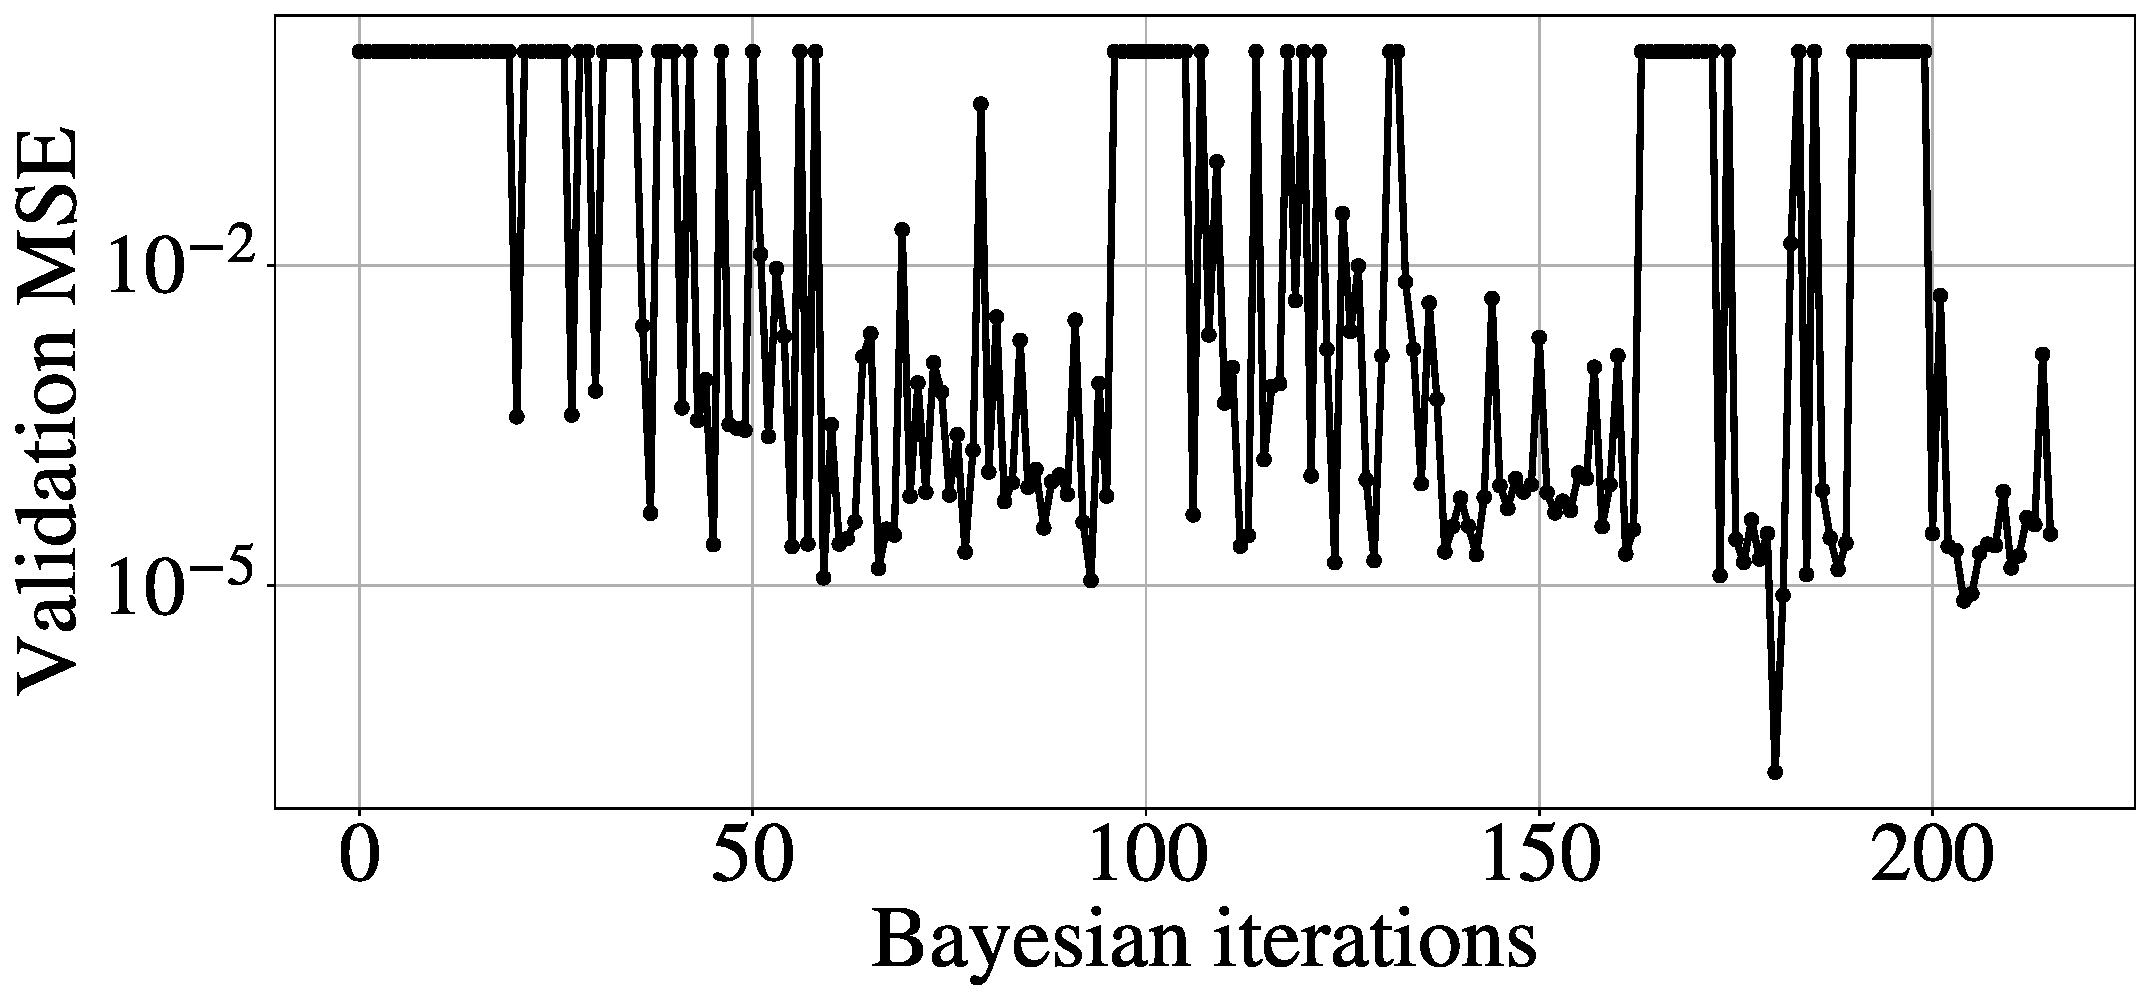
\includegraphics[width=.92\linewidth]{images/nn_nft/scirep_bayes.pdf} (a)
  % \caption{}
  % \label{fig:bayes}
\end{minipage}%
\begin{minipage}{.49\textwidth}
  \centering
  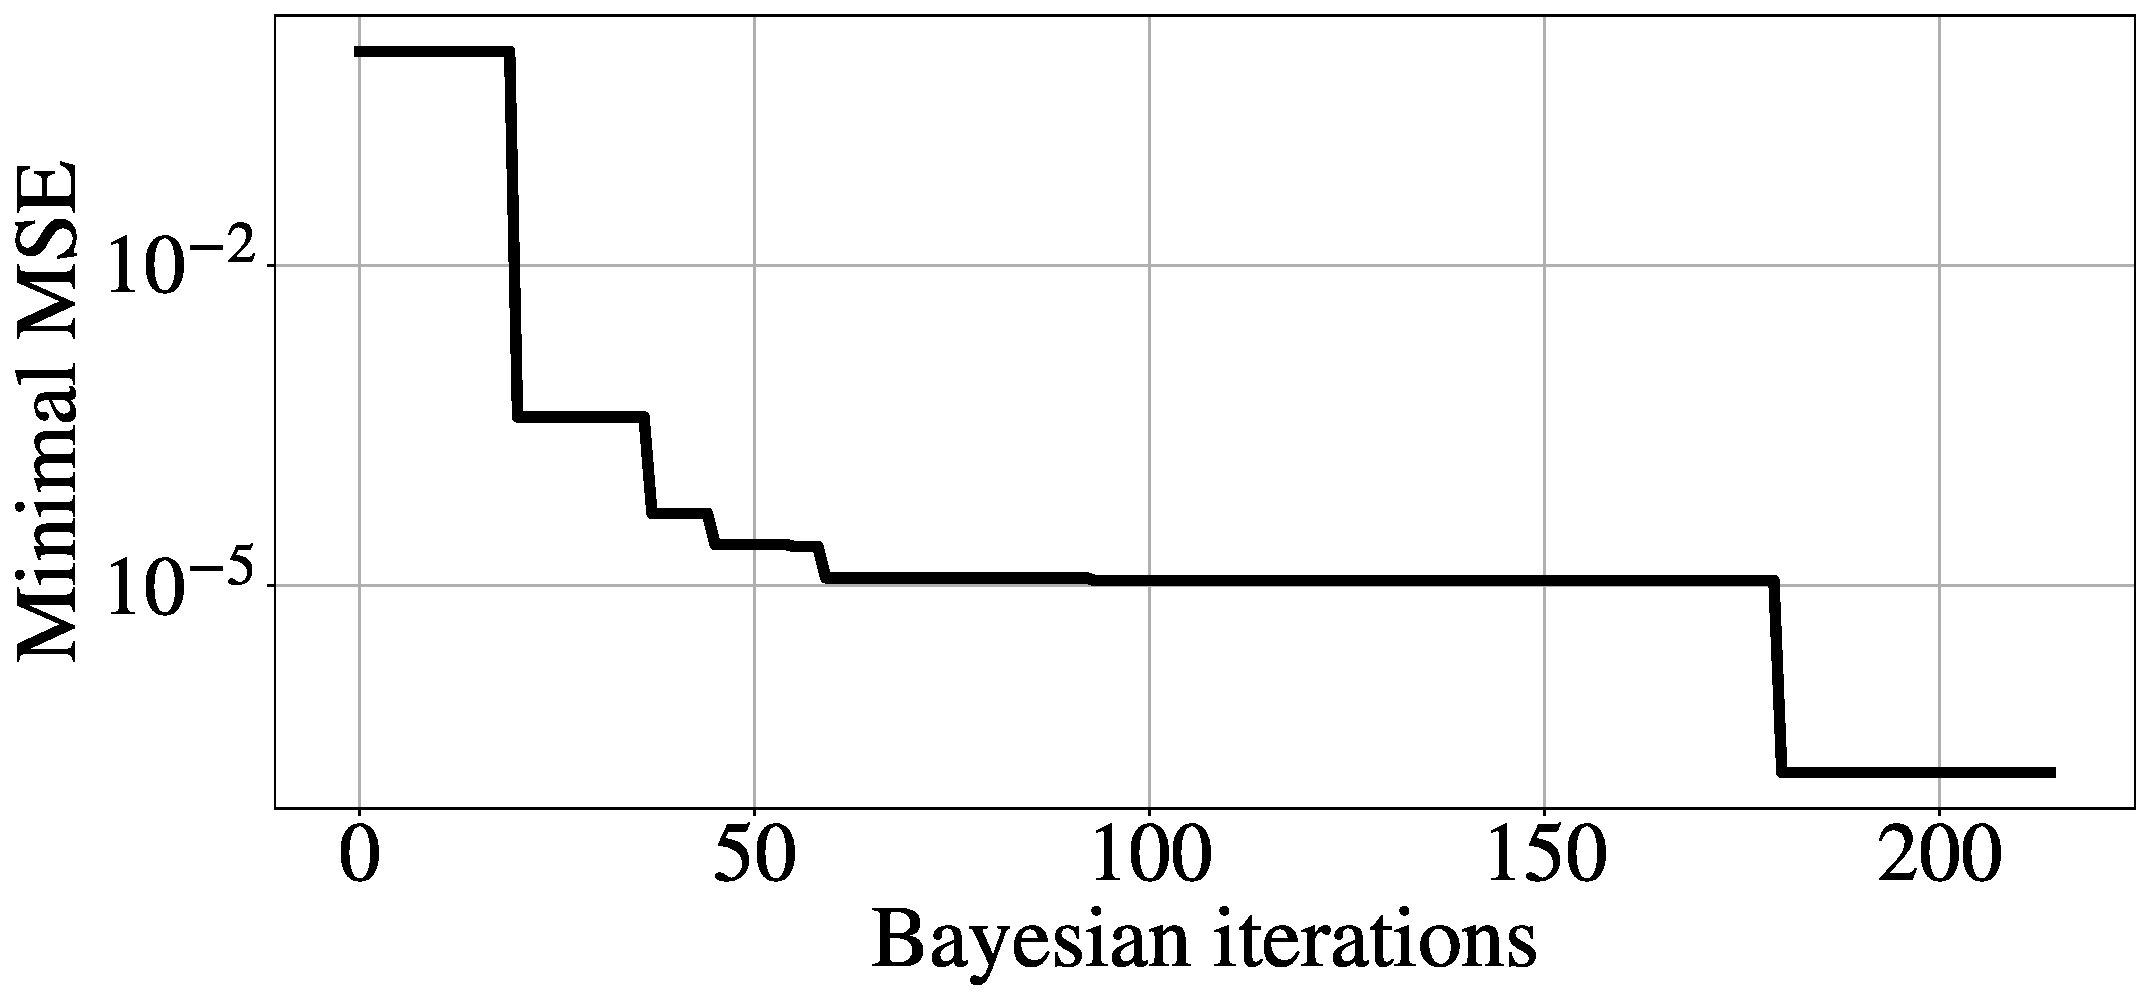
\includegraphics[width=.92\linewidth]{images/nn_nft/scirep_bayes_min.pdf} (b)
  % \caption{}
  % \label{fig:bayes_min}
\end{minipage}
\caption{\textbf{(a)} The dependence of the mean squared error (MSE) value on the number of Bayesian iteration. \textbf{(b)} The same for minimal value of MSE.}
\label{fig:bayes_full}
\end{figure}


The Bayesian optimization builds a probabilistic model of the function mapping from hyperparameter values to the objective evaluated on a validation set\cite{mockus1975bayesian,pelikan1999boa}. By iteratively evaluating a promising hyperparameter configuration based on the current model, and then updating it, the Bayesian optimization aims to gather observations revealing as much information as possible about this function and, in particular, the location of the optimum. Thus, it tries to balance exploration (hyperparameters for which the outcome is most uncertain) and exploitation (the hyperparameters expected to bring us close to the optimum).
An important aspect to note is that the Bayesian optimisation often does not return one specific point in the parameter hyperspace for which the optimised function is minimal. The process converges into some subspace of parameters, where several points can locally minimize the function\cite{pelikan1999boa}.

\begin{figure}[tbph]
    \centering
    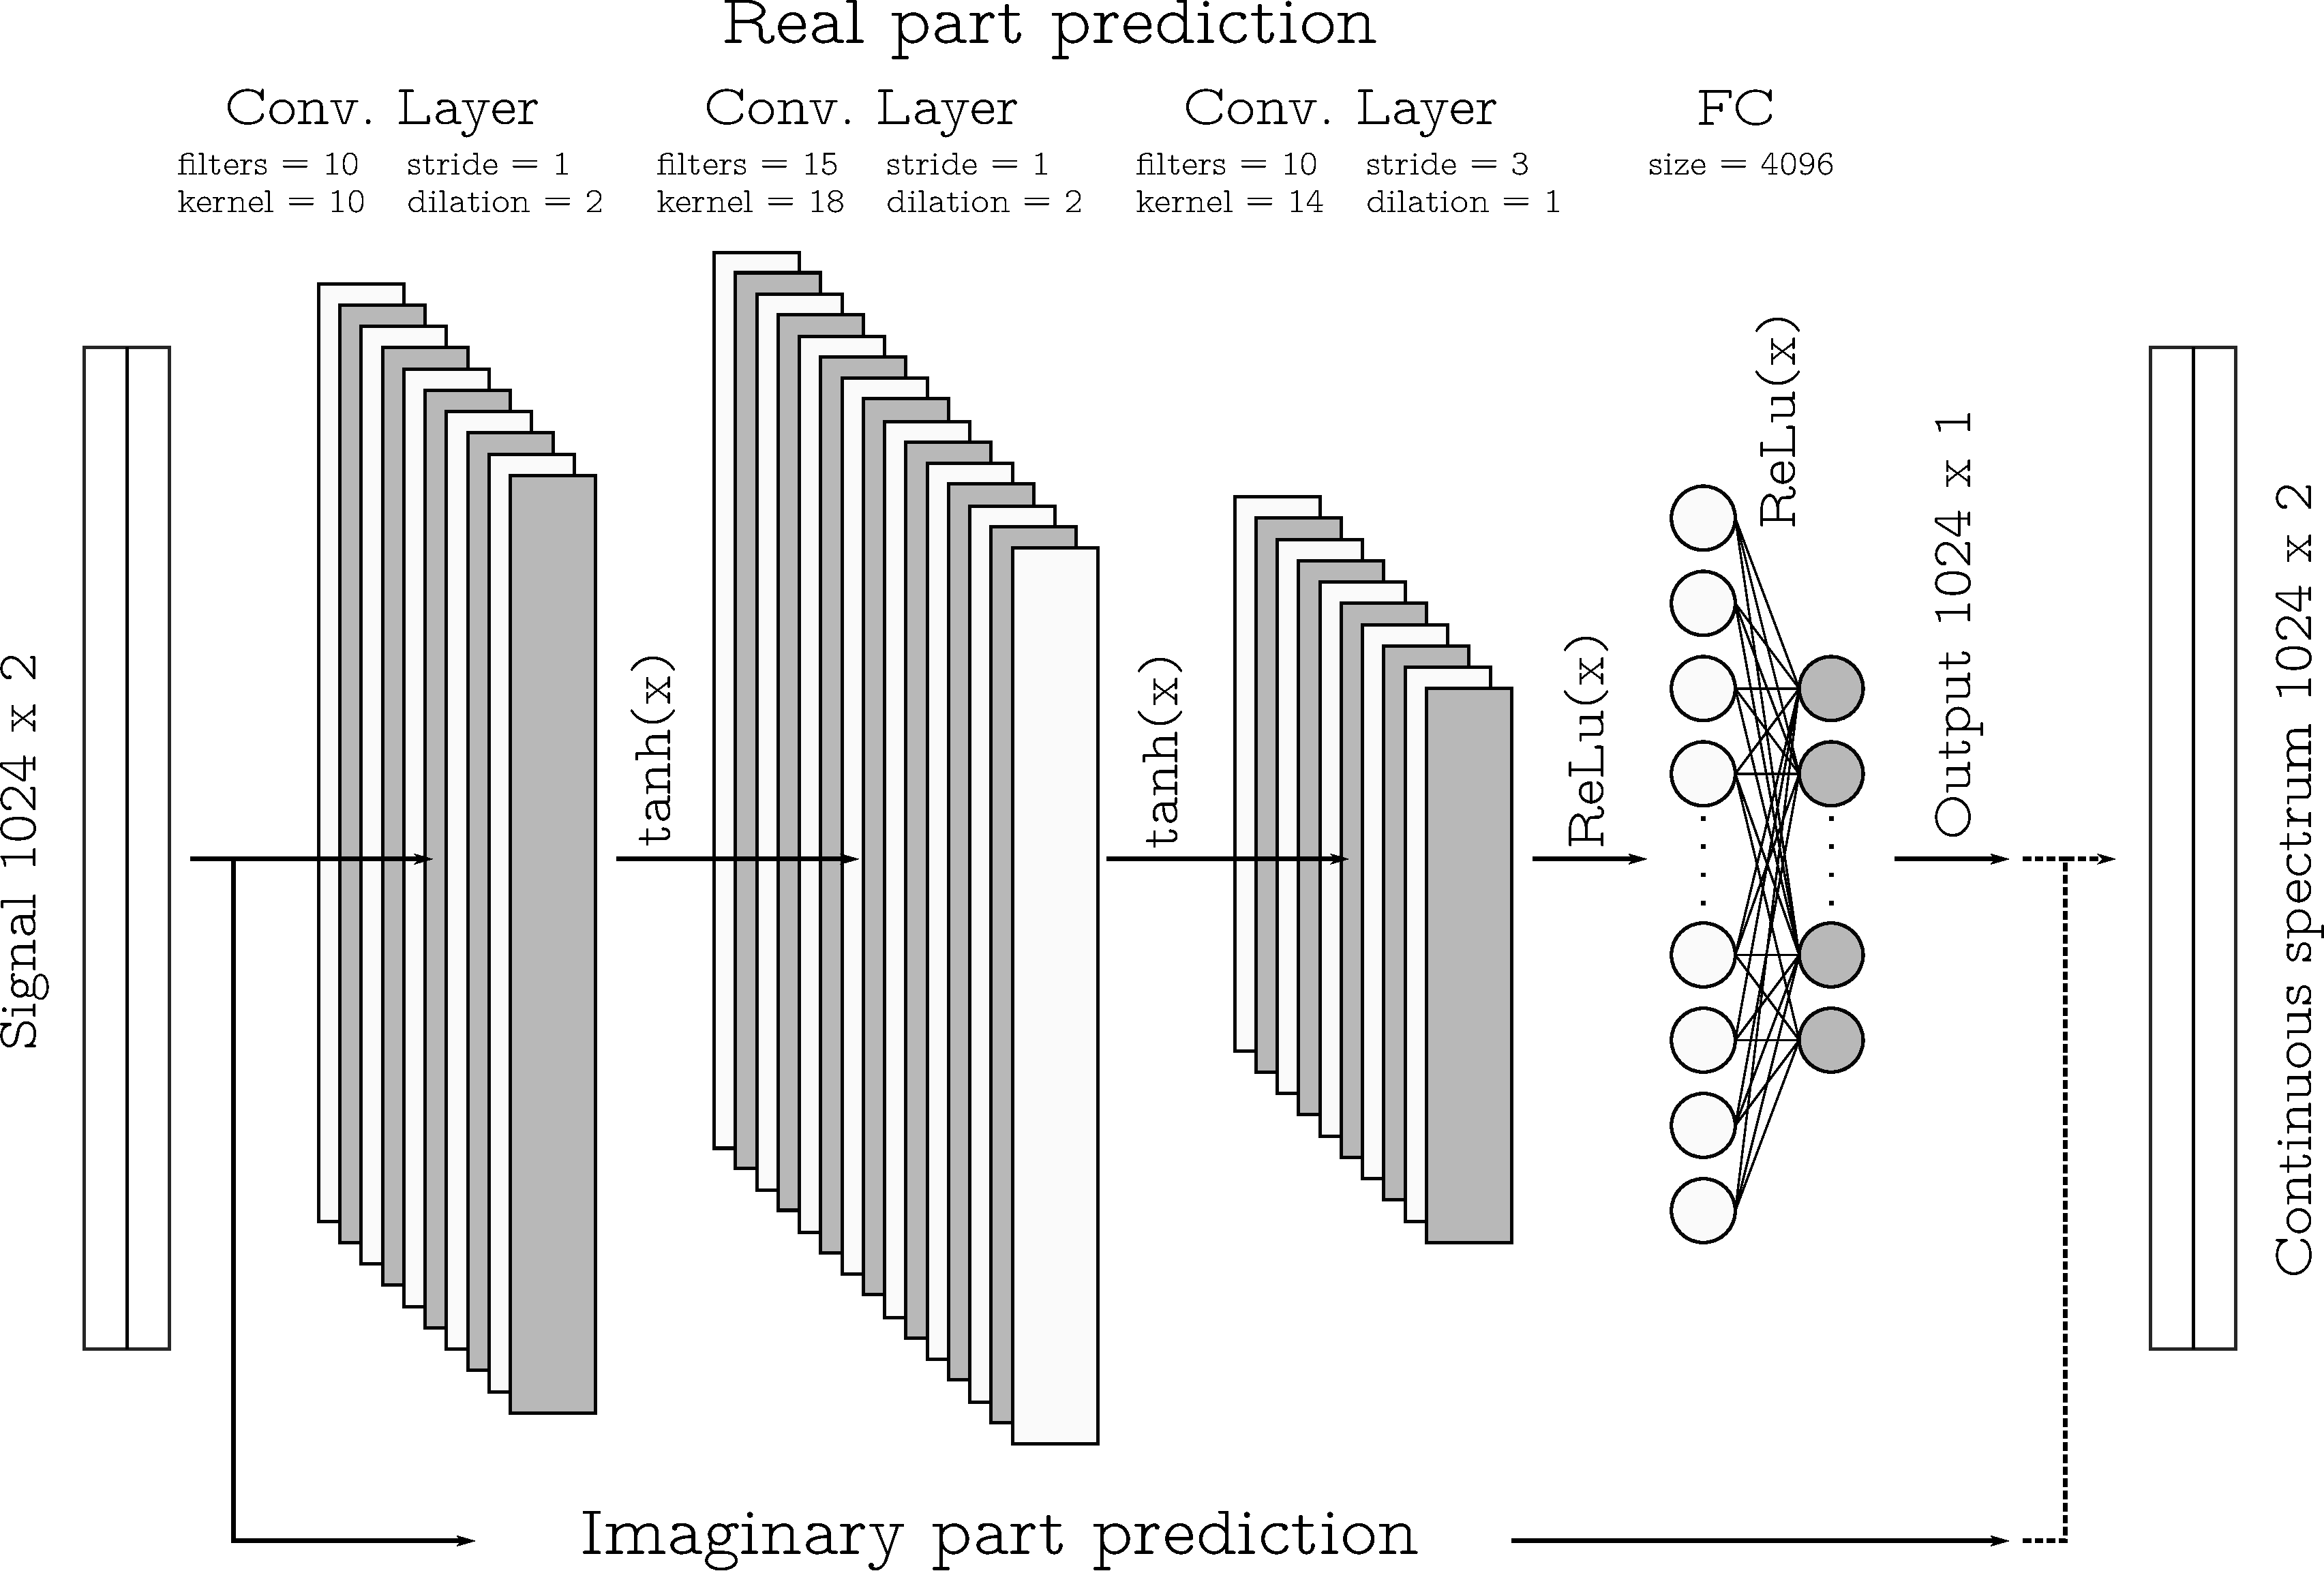
\includegraphics[width=1.0\linewidth]{images/nn_nft/arch_new.pdf}
    \caption{The schematic of NFT-Net topology: the extended scheme presents the sequence of operations for the processing of real part; the processing of imaginary part is identical (marked with the long arrow below the scheme). The numbers indicating the layers/arrays sizes refer to our processing 1024 complex-valued signal samples.}
    \label{fig:nn_architecture}
\end{figure}

% Part about how we did it

We manipulate the following hyperparameters for the convolutional part of the neural network: the number of convolutional layers, the number of filters, the kernel size, stride, dilation, and the activation function for each layer. After the convolutional part, there are 2 fully connected layers, the second of which has a fixed size (1024, which corresponds to the size of the output vector). The size and activation function of the first fully connected layer was also a hyperparameter for optimization.
For the optimisation, we used a dataset without additional noise and employed only the real part of the continuous spectrum for the prediction. After that, the ``optimal'' architecture (but not weights) is fixed, and is no longer changed to predict the imaginary part of the continuous spectrum or for our operating with the datasets with additional noise.
The loss function was optimised for each architecture. We used the mean squared error (MSE) as the loss function, aiming to minimise the MSE between the network output and the target output computed with the conventional NFT method\cite{FNFT2018}. In training, we employed the Adam (Adaptive Moment Estimation) optimisation algorithm with the learning rate of 1e-4 \cite{s2000adaptive}. 
The learning process of each point in the parameter hyperspace was stopped if the value of the loss function did not decrease over 5000 epochs. 
We chose this large epoch stopping-criterium number to neutralise the factor of randomness in the learning process, which appears due to the random choice of the initial weights. Additionally, we checked the value of the loss function on the validation set to prevent the overfitting, but for the amount of training data used, the overfitting was not observed. 
Figure~\ref{fig:bayes_full} presents the dependence of the MSE value and dependence of its minimum on the  Bayesian iteration number. For architectures with more than 20 million training parameters, we set the value of the loss function to $1.0$: this explains the upper cut-off limit in the figure. It is apparent from Fig.~\ref{fig:bayes_full} that the optimisation has identified a subspace where many architectures have approximately the same value of the loss function at the level of $10^{-5}$. However, there was a point where the value was at the level of $10^{-7}$. Thus, we took this point (a set of hyperparameters) as the optimal one.
After finding the optimal architecture, each NN's weights were trained for different SNR but keeping the same optimal architecture parameters. On average, with the amount of data used, our learning process took 50 000 epochs to reach the minimum for each noise level.

% End of the optimisation part

The original signal and NF data for the continuous spectrum are complex-valued functions. Therefore, two networks with the same architecture are to be used for the whole transformation; each identical part is responsible for the computation of either the real or imaginary parts of the resulting arrays, which contain the values of continuous NF spectrum defined in~Eq.~(\ref{r}).  Fig.~\ref{fig:nn_architecture} depicts the schematic for the entire optimised NFT-Net architecture. The convolutional part consists of three layers with 10, 15 and 10 filters. Kernel sizes of the first and third convolutional layers are 10, and for the layer between them, it is 18. As noted above, we took the dilation value for each layer as one of the sought hyperparameters. For NFT-Net, the optimisation gave that the first two layers have dilation 2, stride 1 and ``tanh'' activation function, and for the third layer, the dilation is 1 with stride 3 and ``ReLu''  activation. After the CNN part we put the flattening layer, not shown in the figure (but affecting the processing complexity), and two fully-connected layers with 4096 and 1024 neurons. The exemplary picture of how the designed NN works on one signal is given in Fig.~\ref{fig:won_spectrum}. In this figure, we show the results of the NN-based NF spectrum computation for the noiseless case. Already from this figure, we can notice that the result produced by our NN and that obtained from conventional NFT routine\cite{FNFT2018} are very similar. 


\subsection*{Studying the NFT-Net performance for computing NF spectra of noisy signals}

In this section we analyse the NFT-Net performance and the denoising property of the NN. We compare the deviations in the obtained nonlinear spectrum calculated with the NFT-Net and calculated with the conventional NFT applied to the same signal without noise. To quantify the performance rendered by the NFT-Net application with the performance of conventional algorithms applied to noisy signals, we use the following metric:
\begin{equation}
    \eta = \frac{1}{S} \, \sum_{i = 1}^{S} \langle \eta_i(\xi) \rangle_{\xi},
    \quad
    \eta_i(\xi) = \frac{|\{r_\text{predicted}(\xi)\}_i - \{r_\text{actual}(\xi)\}_i| }{\langle |\{r_\text{actual}(\xi)\}_i| \rangle_{\xi}} {,}
    \label{eq:metric}
\end{equation}
where $S$ is the total number of signals in the validation set, $\langle \cdot \rangle_{\xi}$ denotes the mean over the spectral interval, 
$\{r_{\text{predicted}}(\xi)\}_{i}$ and $\{r_{\text{actual}}(\xi)\}_{i}$ correspond to the value of reflection coefficient $r(\xi)$ computed for the signal number $i$ at point $\xi$ (we compare the quantities for the validation data set).  The label ``predicted'' refers to the result produced by the NFT-Net on the noisy signal, and ``actual'' marks the $r(\xi)$ value obtained using the conventional NFT algorithm\cite{FNFT2018} for the noiseless signal.
The relative error $\eta(\xi)$ is determined at the point $\xi$, so we use $\langle \eta(\xi) \rangle_{\xi}$ to estimate the overall mean of the error for one signal, and use Eq.~(\ref{eq:metric})  to evaluate the error for the entire validation dataset.
We stress that the metric was chosen in such a way as to take into account even the regions where the value of the spectrum is much less than one.


\begin{figure}[htbp]
\centering
\begin{minipage}{.47\textwidth}
  \centering
  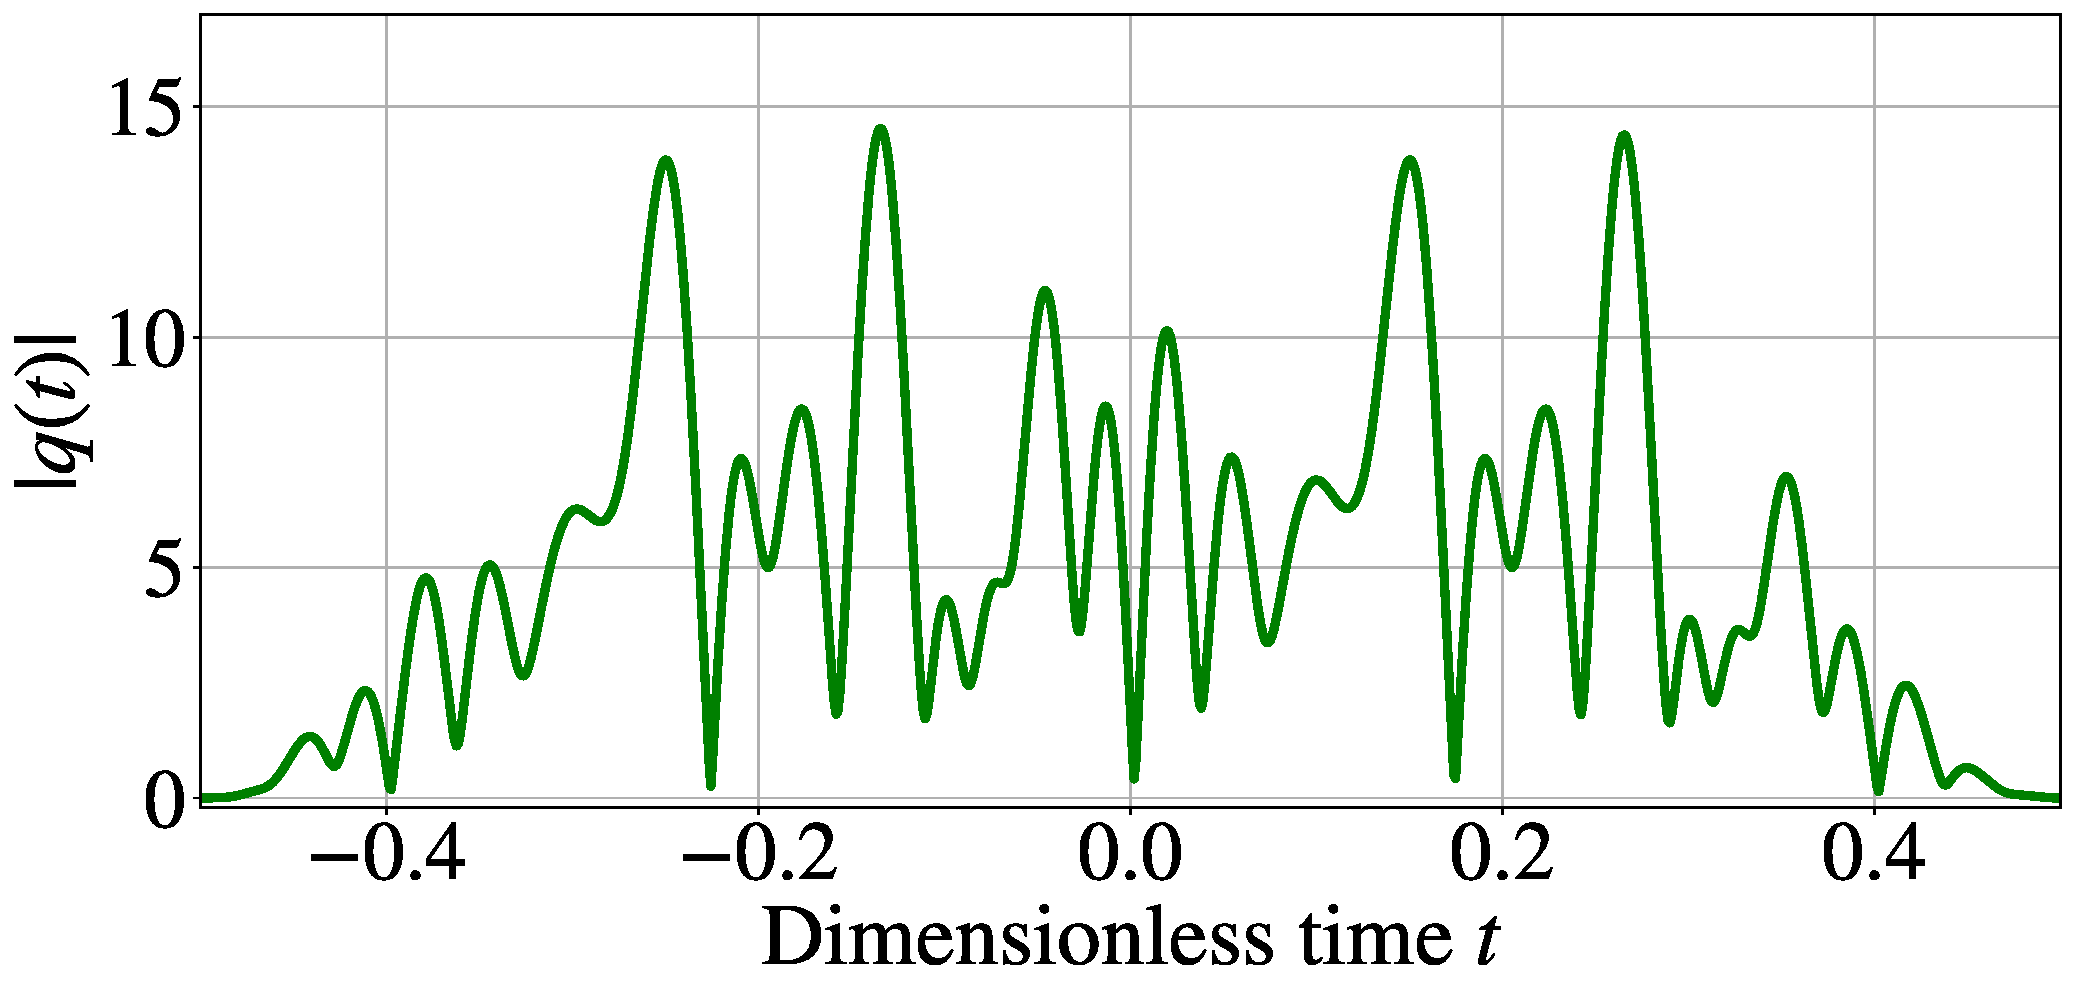
\includegraphics[width=1.\linewidth]{images/nn_nft/scirep_signal_example.pdf}
  \caption{Amplitude of original signal}
  \label{fig:won_signal}
\end{minipage}%
\hfill
\begin{minipage}{.47\textwidth}
  \centering
  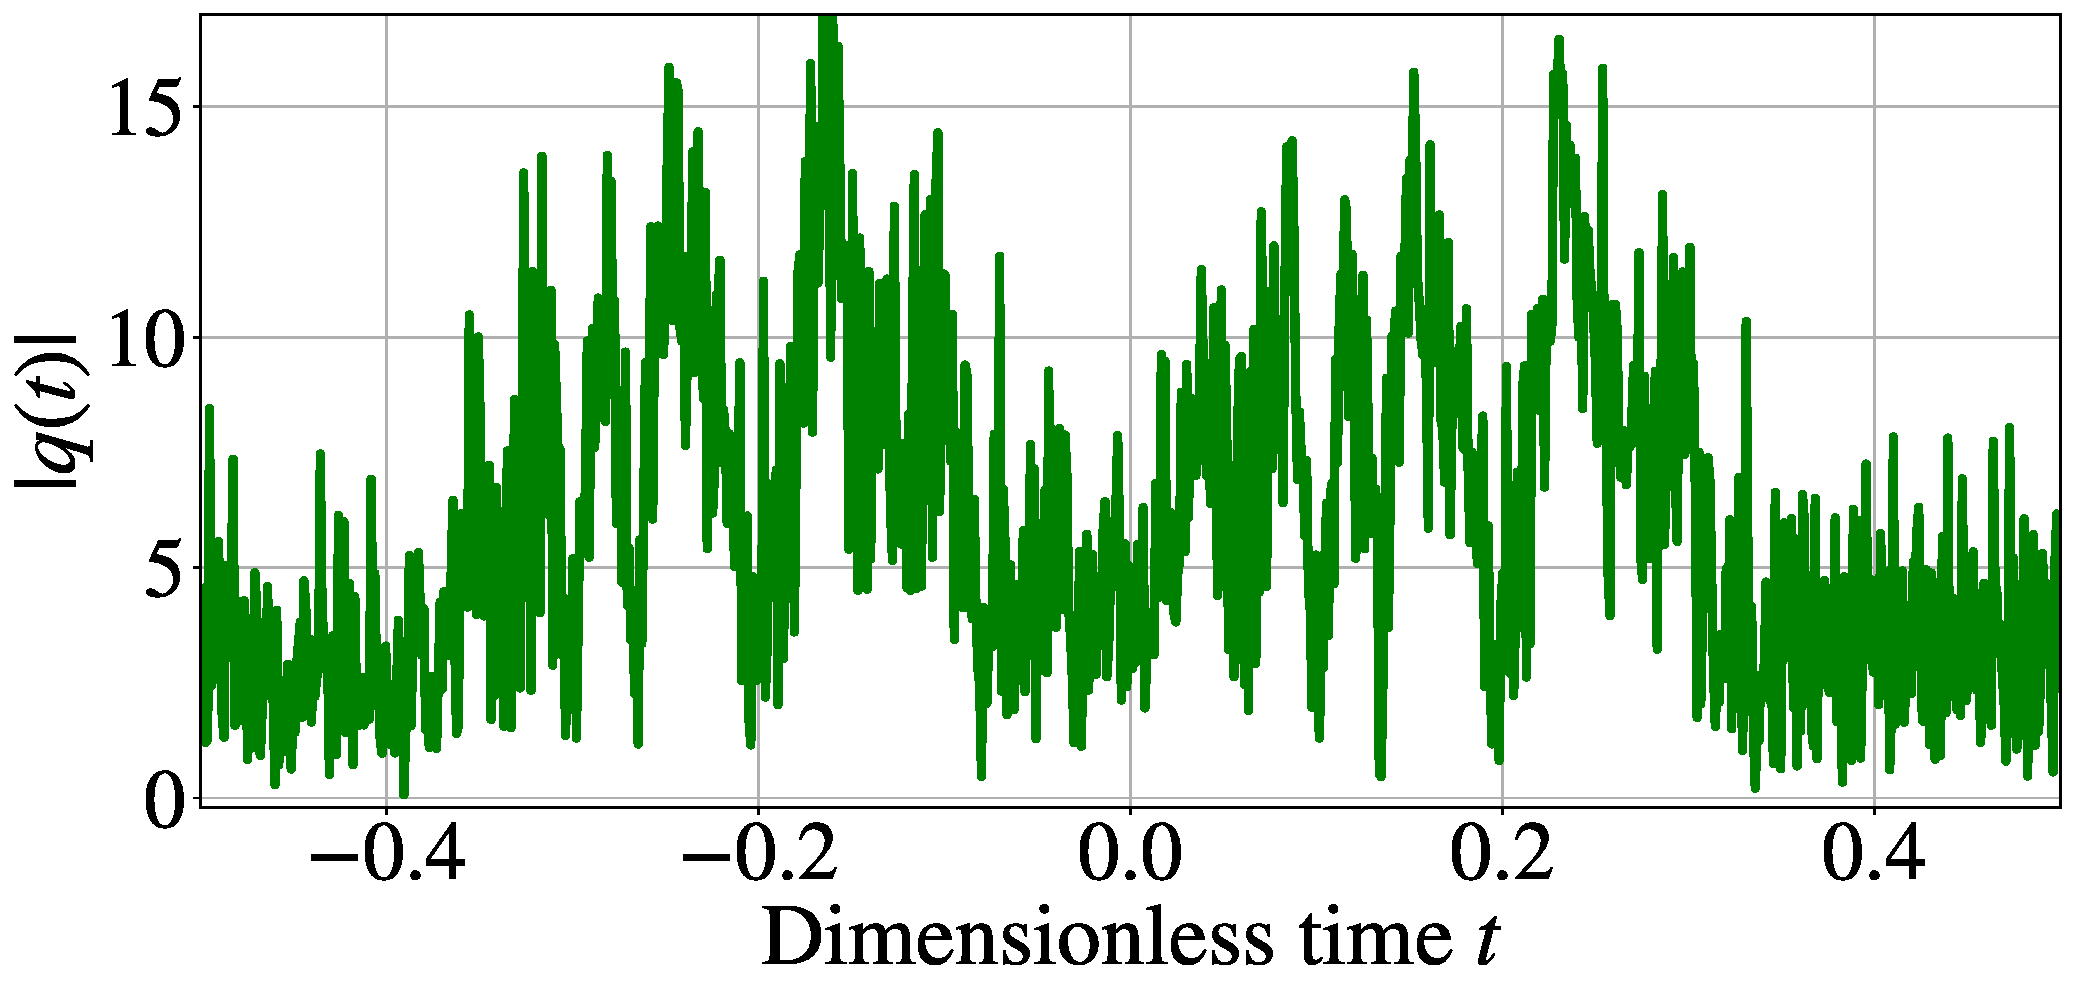
\includegraphics[width=1.\linewidth]{images/nn_nft/scirep_signal_wn_example.pdf}
  \caption{Amplitude of signal with additional noise}
  \label{fig:wn_signal}
\end{minipage}
\\

\begin{minipage}{.47\textwidth}
  \centering
  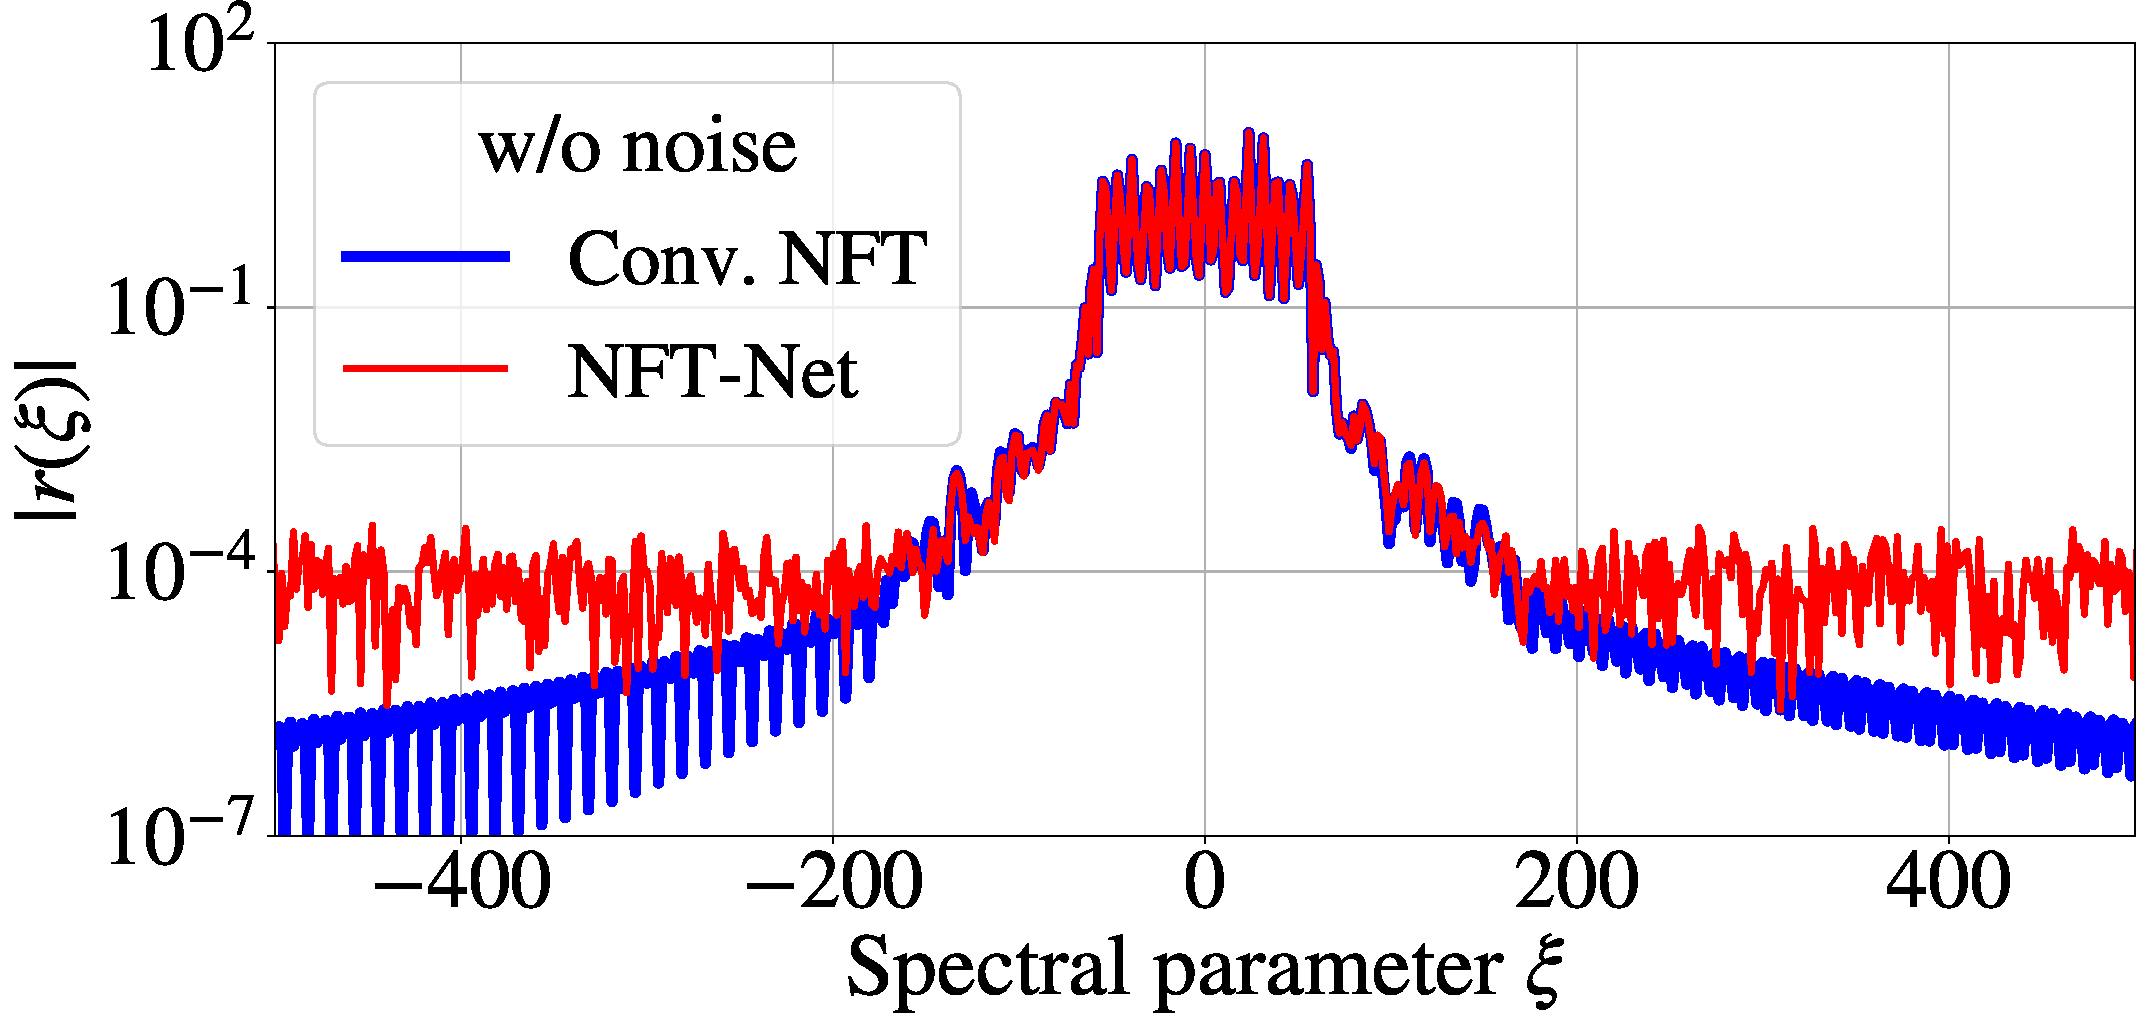
\includegraphics[width=1.\linewidth]{images/nn_nft/scirep_cont_spec_example.pdf}
  \caption{Amplitude of reflection coefficient for continuous spectrum}
  \label{fig:won_spectrum}
\end{minipage}
\hfill
\begin{minipage}{.47\textwidth}
  \centering
  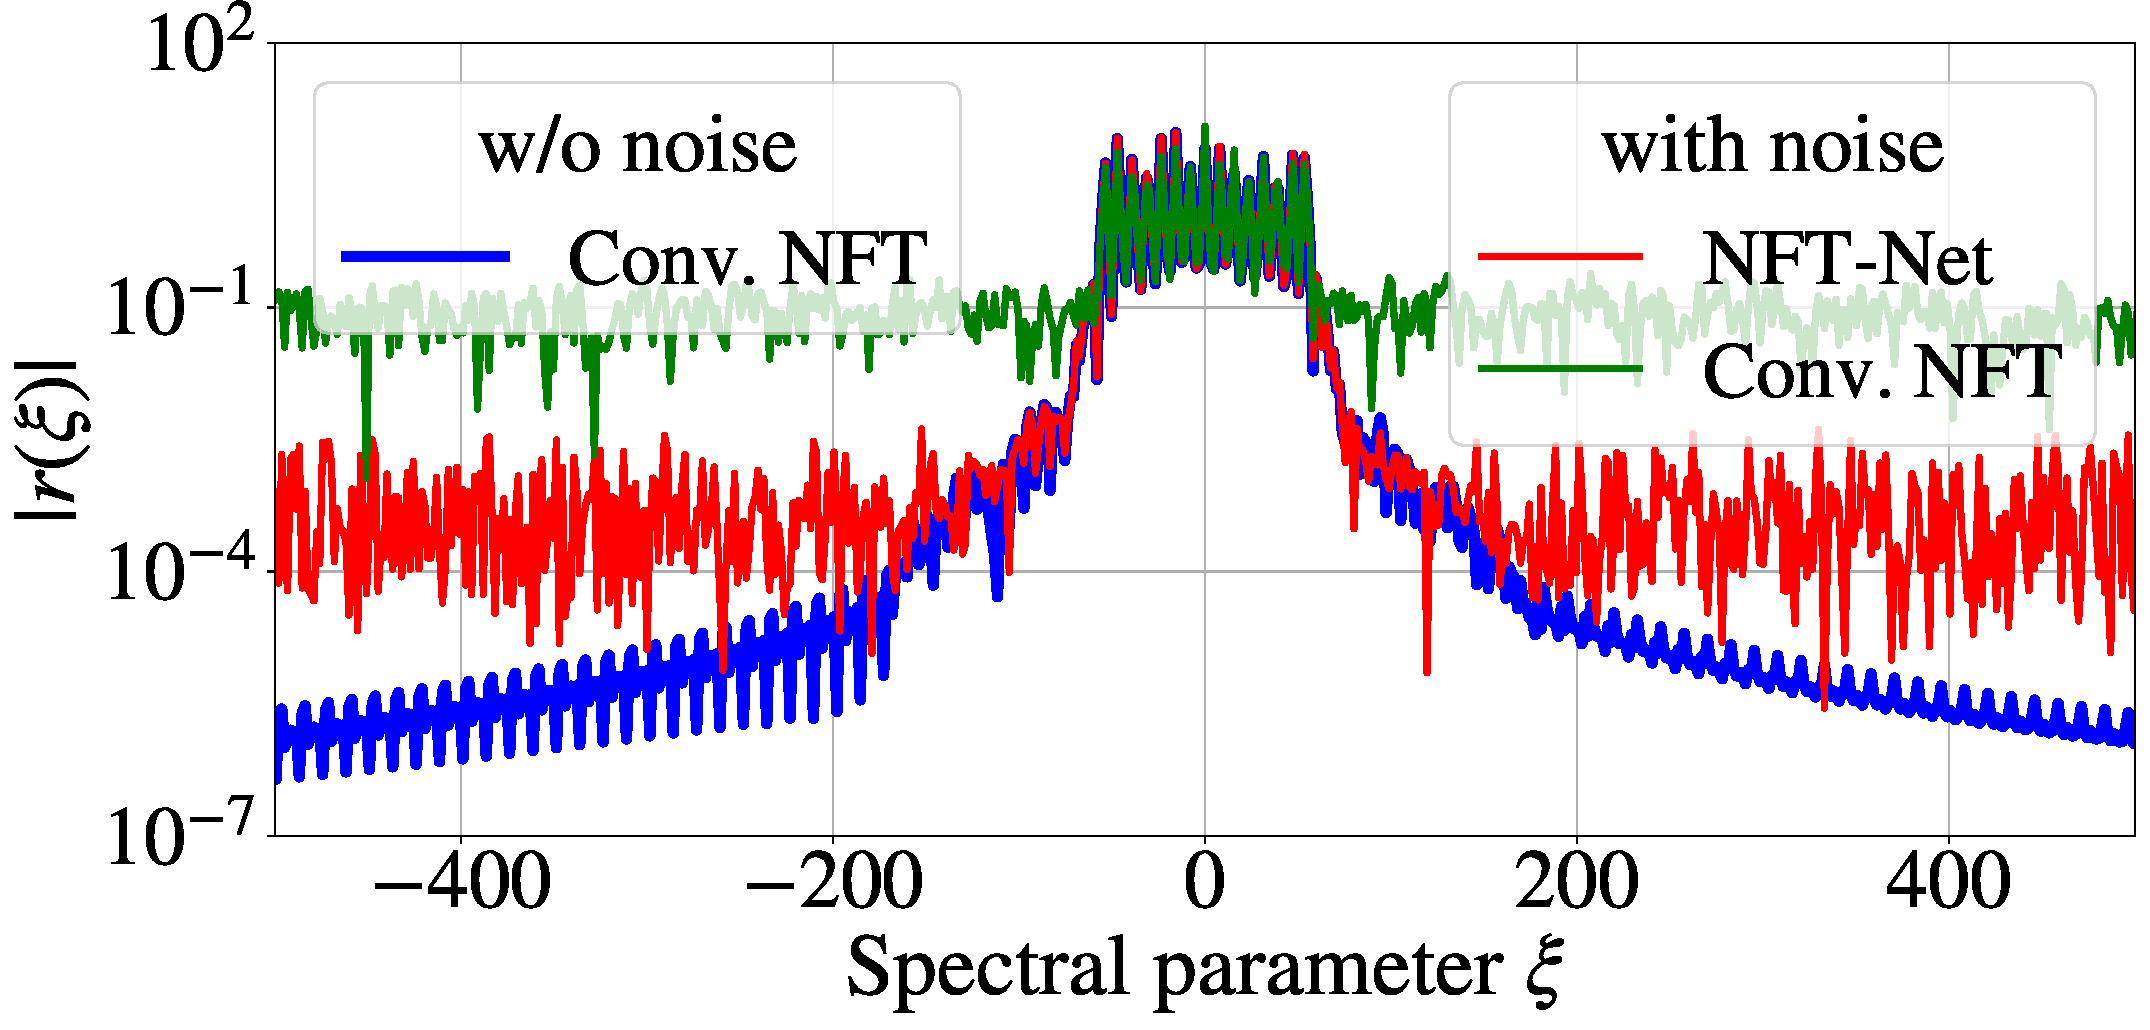
\includegraphics[width=1.\linewidth]{images/nn_nft/scirep_cont_spec_wn_example.pdf}
  \caption{Amplitude of reflection coefficient for continuous spectrum}
  \label{fig:wn_spectrum}
\end{minipage}
\\

\begin{minipage}{.47\textwidth}
  \centering
  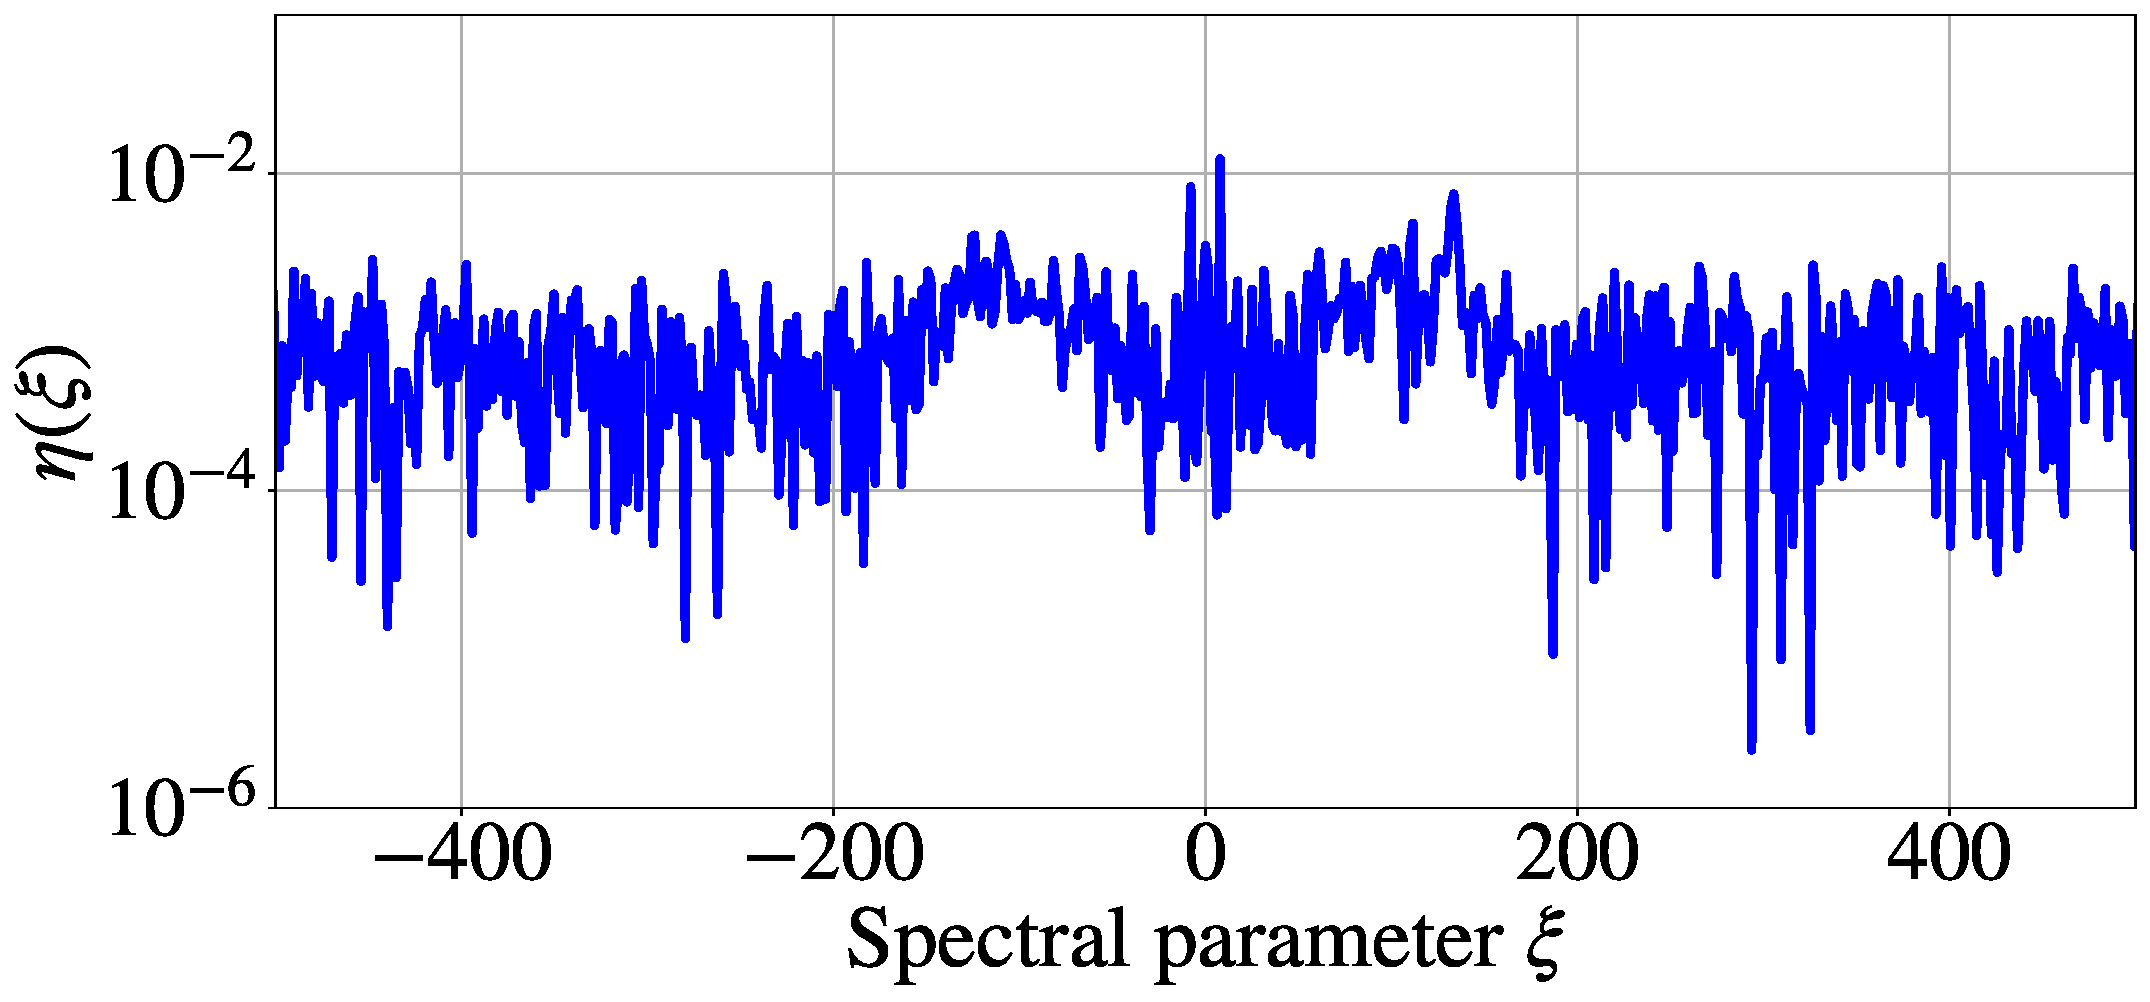
\includegraphics[width=1.\linewidth]{images/nn_nft/scirep_spectrum_diff_example.pdf}
  \caption{Difference between $r(\xi)$ calculated using NFT-Net and Conv. NFT}
  \label{fig:won_diff}
\end{minipage}
\hfill
\begin{minipage}{.47\textwidth}
  \centering
  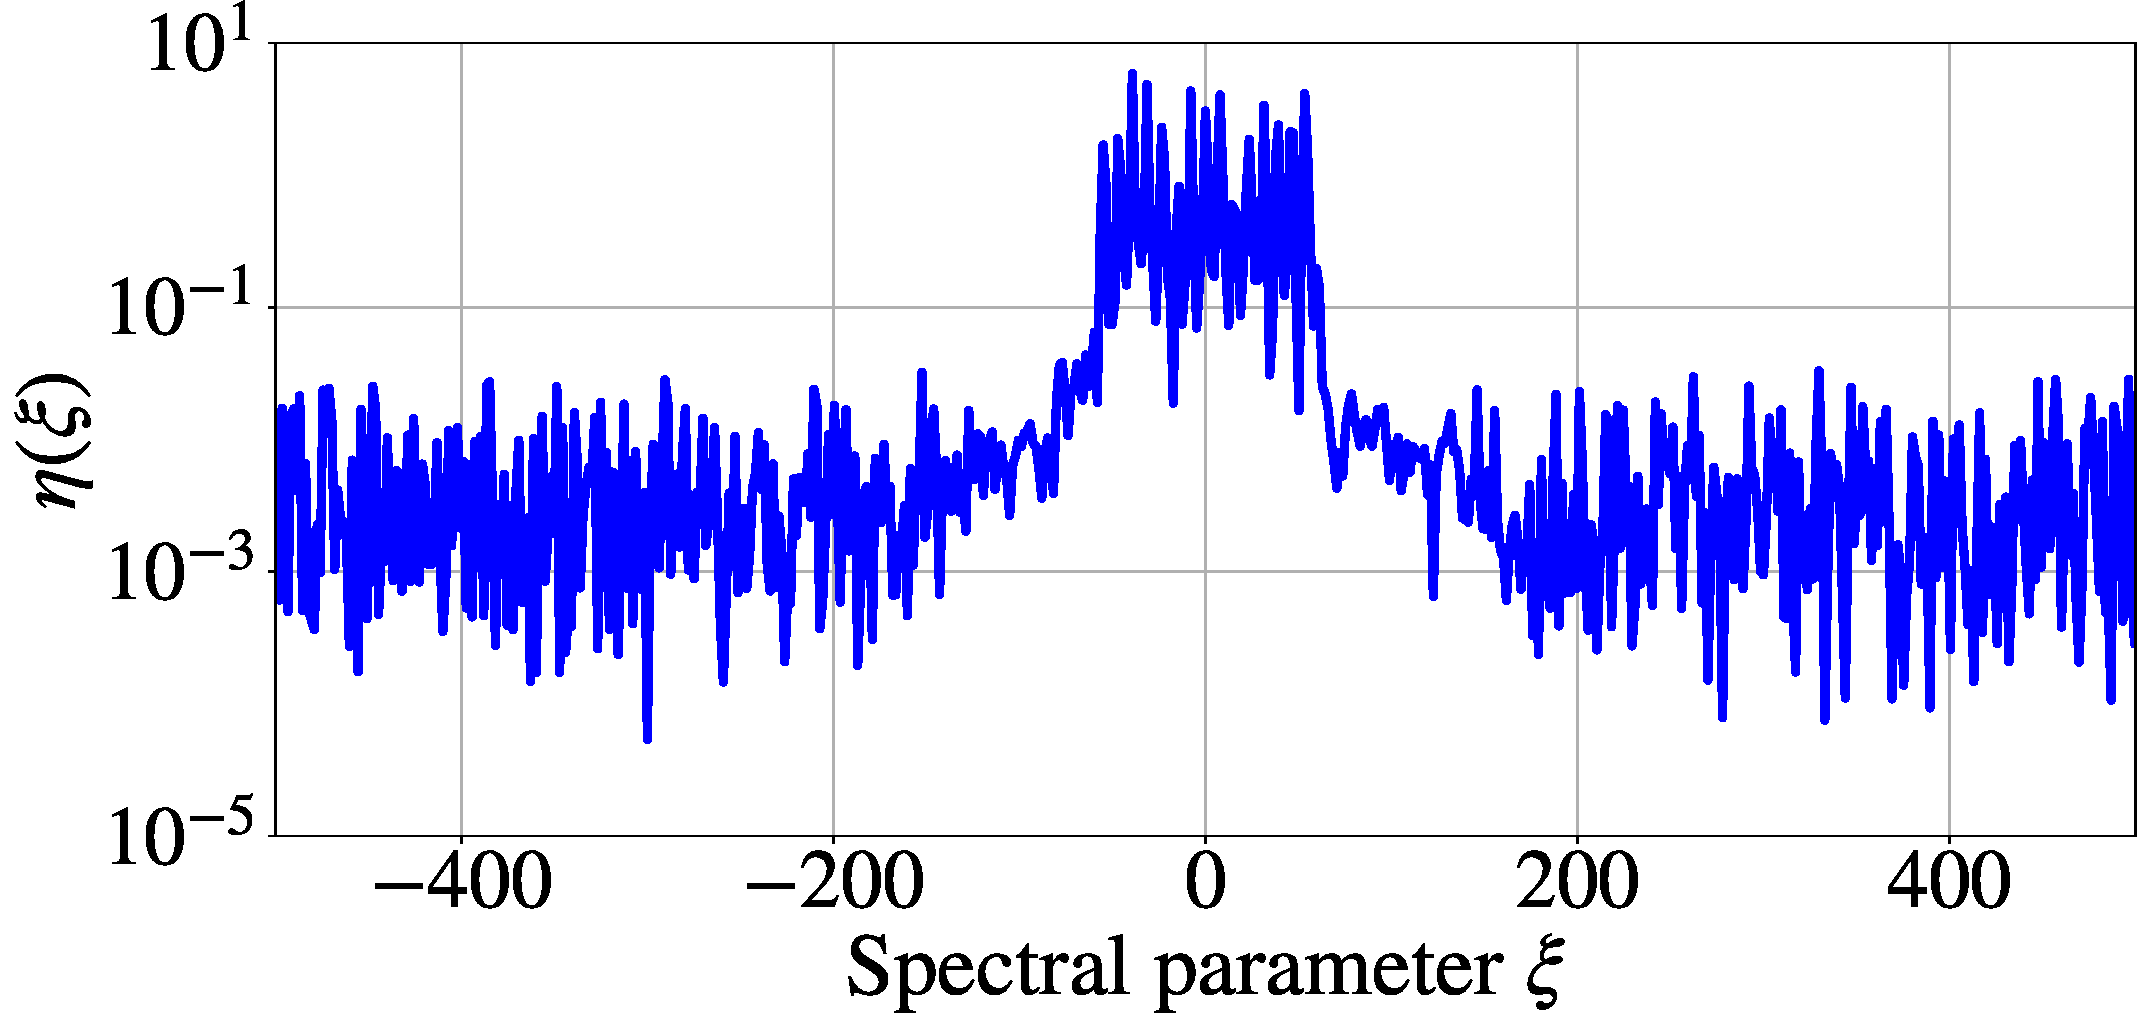
\includegraphics[width=1.\linewidth]{images/nn_nft/scirep_spectrum_diff_wn_example.pdf}
  \caption{Difference between $r(\xi)$ calculated using NFT-Net and Conv. NFT}
  \label{fig:wn_diff}
\end{minipage}


\caption{Panel \textbf{(a)} shows an exemplary amplitude of a original complex WDM signal $q(t)$ versus time. Below (panel \textbf{(c)}) is the amplitude for calculated scattering coefficient $r(\xi)$ associated with the signal from the pane above. The blue line corresponds to the data obtained using the conventional NFT method, the red line corresponds to the NFT-Net result. The difference between the scattering coefficients for signal example calculated by these methods is shown in panel \textbf{(e)}. Pane \textbf{(b)}: the same plot for complex signal $q(t)$ with the addition of Gaussian noise. The SNR value used is 5 dB. Plot \textbf{(d)} shows the result of calculating the continuous spectrum for the noisy signal using the FNFT method (green line) and using the NFT-Net trained at the same noise level (SNR = 5 dB, red line) and original spectrum (for noiseless case, blue line). For NFT-Net trained with noise, pane \textbf{(f)} below shows the difference between the predicted scattering data for the example of noisy signal and the reflection coefficient calculated by conventional NFT for that signal without noise.}
\label{fig:wdm_and_spectrum}
\end{figure}


The results of our comparison for $r(\xi)$ computation using different SNR levels for NFT-Net are presented in Table \ref{tab:nn_with_nft}, and are arranged as follows. The first column of the table identifies the SNR value in dB for the validation signals, i.e. the level of noise for the signals which we analyse. The first row of the table displays the SNR values of noisy signals from the training set, i.e. it shows the noise level of the signals on which the NFT-Net was trained. We notice that the case $\text{SNR}=30$ dB corresponds to almost negligible noise, while for $\text{SNR}=0$ dB our noise energy is equal to that of our signal, which signifies a very intensive noisy corruption. Thus, each column in the table corresponds to the results produced by the NN trained on the signals with the chosen level of a noisy corruption.
The number in each cell shows the averaged metric value, Eq.~(\ref{eq:metric}), where for the computation of $\{r_{\text{predicted}}(\xi)\}_{i}$ we used the NFT-Net trained on the signals with SNR values shown in the first row and applied to the validation signals having the SNR values given in the first column. The ``Conv. NFT'' column shows the error value for the numerical result of the fast NFT method on the signals with added noise, where the respective SNR is presented, again, in the first column. The value of metric~(\ref{eq:metric}) corresponding to the conventional NFT method applied to noiseless signals is, obviously, zero: the results provided by the conventional NFT without noise are taken as the true ones. 
When the NFT-Net produces a less accurate result compared to the conventional NFT applied to the noisy signal, the cell is marked with grey shadowing; when the NFT-Net outperforms the conventional NFT method, i.e. it successfully purifies our signal from noise, the respective cell is not highlighted (white). 
Whence, the white area size in each table demonstrates how well the NFT-Net retrieves the nonlinear spectrum for noise-corrupted signals.


% Table 6x2 linear
\begin{table}[h!]
\centering
\resizebox{1.\textwidth}{!}
{
\begin{tabular}{ >{\columncolor{White}}p{0.001\linewidth}  >{\columncolor{White}}c | >{\columncolor{White}}c | c c c c c c c c c}

% \begin{tabular}{p{0.001\linewidth} c | c | c c c c c c c c c}
  
  & & & \multicolumn{9}{c}{Training SNR level, dB} \\
  
  & & Conv. NFT & w/o noise & 30 & 25 & 20 & 17 & 13 & 10 & 5 & 0 \\
  \hline
  \rowcolor{LightGray} \cellcolor{White} &
  \cellcolor{White} w/o noise & \cellcolor{White} 0 & 8.39e-4 & 6.52e-3 & 9.43e-3 & 1.26e-2 & 1.61e-2 & 2.38e-2 & 3.59e-2 & 7.43e-2 & 1.42e-1 \\
  
  &
  30 & 6.91e-2 & 5.54e-2 & 9.56e-3 & 1.11e-2 & 1.36e-2 & 1.68e-2 & 2.42e-2 & 3.63e-2 & \cellcolor{LightGray} 7.49e-2 & \cellcolor{LightGray} 1.44e-1 \\

  &
  25 & 1.23e-1 & 9.84e-2 & 1.40e-2 & 1.39e-2 & 1.51e-2 & 1.78e-2 & 2.45e-2 & 3.63e-2 & 7.47e-2 & \cellcolor{LightGray} 1.43e-1 \\

  &
  20 & 2.21e-1 & 1.74e-1 & 2.53e-2 & 2.18e-2 & 1.97e-2 & 2.08e-2 & 2.58e-2 & 3.65e-2 & 7.40e-2 & 1.43e-1 \\

  &
  17 & 3.10e-1 & 2.41e-1 & 3.96e-2 & 3.23e-2 & 2.63e-2 & 2.53e-2 & 2.78e-2 & 3.70e-2 & 7.31e-2 & 1.42e-1 \\

  &
  13 & 4.89e-1 & 3.66e-1 & 7.74e-2 & 6.12e-2 & 4.53e-2 & 3.97e-2 & 3.54e-2 & 3.98e-2 & 7.06e-2 & 1.38e-1 \\

  &
  10 & 6.78e-1 & 4.88e-1 & 1.29e-1 & 1.03e-1 & 7.36e-2 & 6.23e-2 & 5.12e-2 & 4.85e-2 & 6.87e-2 & 1.33e-1 \\

  & 
  5 & 1.16e+0 & 7.26e-1 & 2.73e-1 & 2.31e-1 & 1.72e-1 & 1.43e-1 & 1.15e-1 & 9.93e-2 & 7.98e-2 & 1.17e-1 \\

  \multirow{-9}{*}{\rotatebox[origin=c]{90}{Validation SNR level, dB}}& 
   0 & 2.00e+0 & 9.48e-1 & 4.79e-1 & 4.37e-1 & 3.60e-1 & 3.12e-1 & 2.59e-1 & 2.29e-1 & 1.74e-1 & 1.16e-1 \\

    
\end{tabular}
}
\caption{Comparison of the NFT-Net performance against the conventional NFT in the computation of coefficient $r(\xi)$. The table presents the results for the optimised NFT-Net architecture from Fig.~\ref{fig:nn_architecture}. The values in the cells show the error value (\ref{eq:metric}) for each specific pair of training and validation sets SNR. The gray cells correspond to the cases when the accuracy of the NFT-Net nonlinear spectrum restoration is lower than that of fast NFT, i.e. the NN does not denoise the signal well, while the white cells correspond to the cases when the accuracy of the continuous NF spectrum rendered by the NFT-Net is higher, i.e. the NN effectively denoises the result.}
\label{tab:nn_with_nft}
\end{table}

Table \ref{tab:nn_with_nft} shows the error values for the restoration of $r(\xi)$ coefficient (\ref{r}) of a noiseless and noisy-perturbed signals (\ref{eq:wdm}), by the NFT-Net architecture given in Fig.~\ref{fig:nn_architecture}. The first row in the table corresponds to the noiseless case. It is always marked with grey, which means that the NN cannot provide any better results than the benchmark ones rendered by the conventional fast NFT method used to generate the training data. 

However, the values of the error for noise-corrupted signals reveal interesting tendencies. 
It follows from the table that for the low training noise level (up to 10 dB, columns three through nine), the NFT-Net error is typically lowest for the noiseless validation dataset (second row).
Thus, the addition of low noise in the training dataset only degrades the NFT-Net restoration capability, even though this decrease is not significant. This NFT-Net feature can be deemed as the NN's being ``confused'' by the weak noise in its training in the nonlinear transformation identification. 
For the most interesting case of high noise, the network works best for samples where the SNR value is the same for the validation and training sets. 
In such cases, the relative error is about 8-12\%, while the error for conventional NFT is at the level of 100-200\%.
Another fact is that with decreasing noise (rows from bottom to top) in the validation set, the error value remains at approximately the same level after the cell corresponding to the same training and validation noise values. 
These results confirm that the presented NN architecture is capable of performing the desired nonlinear transformation, the NFT, and, in addition, it can also work as an effective denoising element when the noise level becomes non-negligible. 



The examples of original and noise-corrupted signals and the corresponding nonlinear continuous spectra are given in Fig.~\ref{fig:wdm_and_spectrum}, where we used the NFT-Net for the computations. Figures~\ref{fig:wn_signal} and~\ref{fig:wn_spectrum} show that when the additional noise distorts the signal, the conventional numerical algorithms naturally produce the noise-distorted nonlinear spectra.
Figs.~\ref{fig:won_diff} and~\ref{fig:wn_diff} show the relative error value $\eta(\xi)$~(\ref{eq:metric}) for the continuous spectrum prediction with NFT-Net for the signal without noise (left) and the signal with noise (right), and the reflection coefficient computed for the original signal by the conventional NFT (marked as ``Conv. NFT'' in the panes' legends). In Figs.~\ref{fig:won_spectrum},~\ref{fig:won_diff}, the NFT-Net is trained on the dataset without adding noise, and in Figs.~\ref{fig:wn_spectrum},~\ref{fig:wn_diff}, the NFT-Net is trained on the dataset with additional noise for SNR = 5 dB. Figs.~\ref{fig:won_spectrum} and~\ref{fig:wn_spectrum} show that in the presence of noise, the fast NFT results begin to deviate noticeably from the original (noiseless) values, while the NFT-Net tends to denoise the resulting nonlinear spectrum.








\subsection*{NFT-Net performance for the restoration of NF coefficient $b(\xi)$ attributed to noisy signals}
In addition to the coefficient $r$, from the optical communications perspective it is instructive and important to check how the proposed architecture would work to predict the NF coefficient $b$, Eq.~(\ref{f:ab}). We note that the optical transmission method coined b-modulation \cite{w17,wsh20,svp20}, where we operate with the modulation of the b-coefficient, has proven to be the most efficacious technique among different NFDM methods proposed \cite{yal19,yla19}. Moreover, for the practical case when our signal has a finite extent, the continuous part of the NF spectrum can be completely described by the b-coefficient only, because the second NF coefficient $a(\xi)$ can be calculated from $b(\xi)$ profile, see Eq.~(\ref{a-fin}) in Methods. Our goal here is to demonstrate that the same NFT-Net structures can be used for the both $r(\xi)$ and $b(\xi)$ computation, when the NN is trained on the respective dataset. As the loss function, we now use the MSE build on the b-coefficient samples, and the MSE is also used as our quality metric in the respective tables:
\begin{equation}
    \eta_b = \frac{1}{S} \, \sum_{i = 1}^{S} \langle \eta_{b,i}(\xi) \rangle_{\xi}, 
    \qquad 
    \eta_{b,i}(\xi) = \frac{|\{b_\text{predicted}(\xi)\}_i - \{b_\text{actual}(\xi)\}_i| }{\langle |\{b_\text{actual}(\xi)\}_i| \rangle_{\xi}}.
    \label{eq:b_metric}
\end{equation}
The notations are the same as we used in~(\ref{eq:metric}): the labels ``predicted'' and ``actual'' correspond, respectively, to the result of the NFT-Net applied to noisy signals and the result produced by the conventional NFT routine applied to noiseless signals.

We carried out the analysis of the NFT-Net performance for the restoration of b-coefficient using the same approach as we did in the previous subsection for $r(\xi)$. Our results for noise pulses with the different level of noise are summarised in Table~\ref{tab:nn_with_nft_b}. 
We checked that the NFT-Net configurations when applied to the computation and denoising of $b(\xi)$ revealed the same tendencies for the quality of restoration as we observed in the previous subsection devoted to the reflection coefficient $r(\xi)$.
\begin{table}[h!]
\centering
\resizebox{1.\textwidth}{!}
{
\begin{tabular}{ >{\columncolor{White}}p{0.001\linewidth}  >{\columncolor{White}}c | >{\columncolor{White}}c | c c c c c c c c c}
  
  & & & \multicolumn{9}{c}{Training SNR level, dB} \\
  
  & & Conv. NFT & w/o noise & 30 & 25 & 20 & 17 & 13 & 10 & 5 & 0 \\
  \hline
  \rowcolor{LightGray} \cellcolor{White} &
  \cellcolor{White} w/o noise & \cellcolor{White} 0 & 7.12e-3 & 5.37e-3 & 5.87e-3 & 6.49e-3 & 8.69e-3 & 1.07e-2 & 1.20e-2 & 1.58e-2 & 1.77e-2 \\
  
  & 30 & 1.15e-1 & 5.83e-2 & 6.73e-3 & 6.69e-3 & 7.16e-3 & 8.95e-3 & 1.08e-2 & 1.20e-2 & 1.58e-2 & 1.77e-2 \\

  & 25 & 2.05e-1 & 1.02e-1 & 1.02e-2 & 8.70e-3 & 8.48e-3 & 9.54e-3 & 1.09e-2 & 1.21e-2 & 1.58e-2 & 1.77e-2 \\

  & 20 & 3.64e-1 & 1.75e-1 & 2.13e-2 & 1.51e-2 & 1.18e-2 & 1.12e-2 & 1.14e-2 & 1.23e-2 & 1.59e-2 & 1.78e-2 \\

  & 17 & 5.14e-1 & 2.38e-1 & 3.66e-2 & 2.41e-2 & 1.59e-2 & 1.33e-2 & 1.21e-2 & 1.26e-2 & 1.60e-2 & 1.78e-2 \\

  & 13 & 8.14e-1 & 3.44e-1 & 7.73e-2 & 4.94e-2 & 2.64e-2 & 1.88e-2 & 1.39e-2 & 1.36e-2 & 1.63e-2 & 1.80e-2 \\

  & 10 & 1.15e+0 & 4.41e-1 & 1.31e-1 & 8.58e-2 & 4.21e-2 & 2.70e-2 & 1.67e-2 & 1.51e-2 & 1.69e-2 & 1.84e-2 \\

  & 5 & 2.04e+0 & 6.22e-1 & 2.70e-1 & 1.96e-1 & 9.95e-2 & 5.91e-2 & 2.81e-2 & 2.18e-2 & 1.95e-2 & 1.99e-2 \\

  \multirow{-9}{*}{\rotatebox[origin=c]{90}{Validation SNR level, dB}} & 0 & 3.60e+0 & 7.98e-1 & 4.54e-1 & 3.68e-1 & 2.24e-1 & 1.42e-1 & 6.34e-2 & 4.43e-2 & 2.93e-2 & 2.43e-2 \\

    
\end{tabular}
}
\caption{Comparison of the NFT-Net performance against the fast conventional NFT in the computation of coefficient $b(\xi)$. The table presents the results for the NFT-Net architecture from Fig.~\ref{fig:nn_architecture}. The values in the cells show the error value (\ref{eq:b_metric}) for each specific pair of training and validation sets SNR. The grey cells correspond to the cases when the accuracy of the NFT-Net nonlinear spectrum restoration is lower than that of fast NFT, i.e. the NN does not denoise the signal well, while the white cells correspond to the cases when the accuracy of the continuous NF spectrum rendered by the NFT-Net is higher, i.e. the NN effectively denoises the signal.}
\label{tab:nn_with_nft_b}
\end{table}
A similar situation as was observed for coefficient $r(\xi)$, remains in this case. The error is minimal for a noiseless validation set. However, this trend now continues for high noise levels.
A similar tendency is observed all over the results: the values above the diagonal vary slightly.
The additional observations when dealing the b-coefficient are as follows. An interesting difference from the case relevant to $r(\xi)$, is that the metric value~(\ref{eq:b_metric}) in the case of predicting $b(\xi)$ is less, and the grey-shadowed region in Table \ref{tab:nn_with_nft} is larger compared to what we see in Table \ref{tab:nn_with_nft_b} for the b-coefficient.
From the results, it is clear that the prediction accuracy is higher for the b-coefficient. 
It means that our NN generally works more accurately for the restoration of coefficient $b(\xi)$ than for $r(\xi)$. This result can be expected, as the noise-perturbed $r(\xi)$ contains the noisy contributions from both $a(\xi)$ and $b(\xi)$, while the b-coefficient involves only its noisy contribution, and thus gets corrupted less. So in the latter case, the NN has to clean off less noise.

Figure~\ref{fig:quality_r_b} summarizes the above and shows the calculation errors~(\ref{eq:metric}) and~(\ref{eq:b_metric})  for NFT-Net architecture. The plot actually visualises the values and tendencies from Tables \ref{tab:nn_with_nft} and \ref{tab:nn_with_nft_b}. For both $r(\xi)$ and $b(\xi)$ coefficients, the NN outperforms the fast NFT results when the NFT-Net gets trained on the data with additional noise. 


\begin{figure}[tp]
\centering
\begin{minipage}{.49\textwidth}
  \centering
  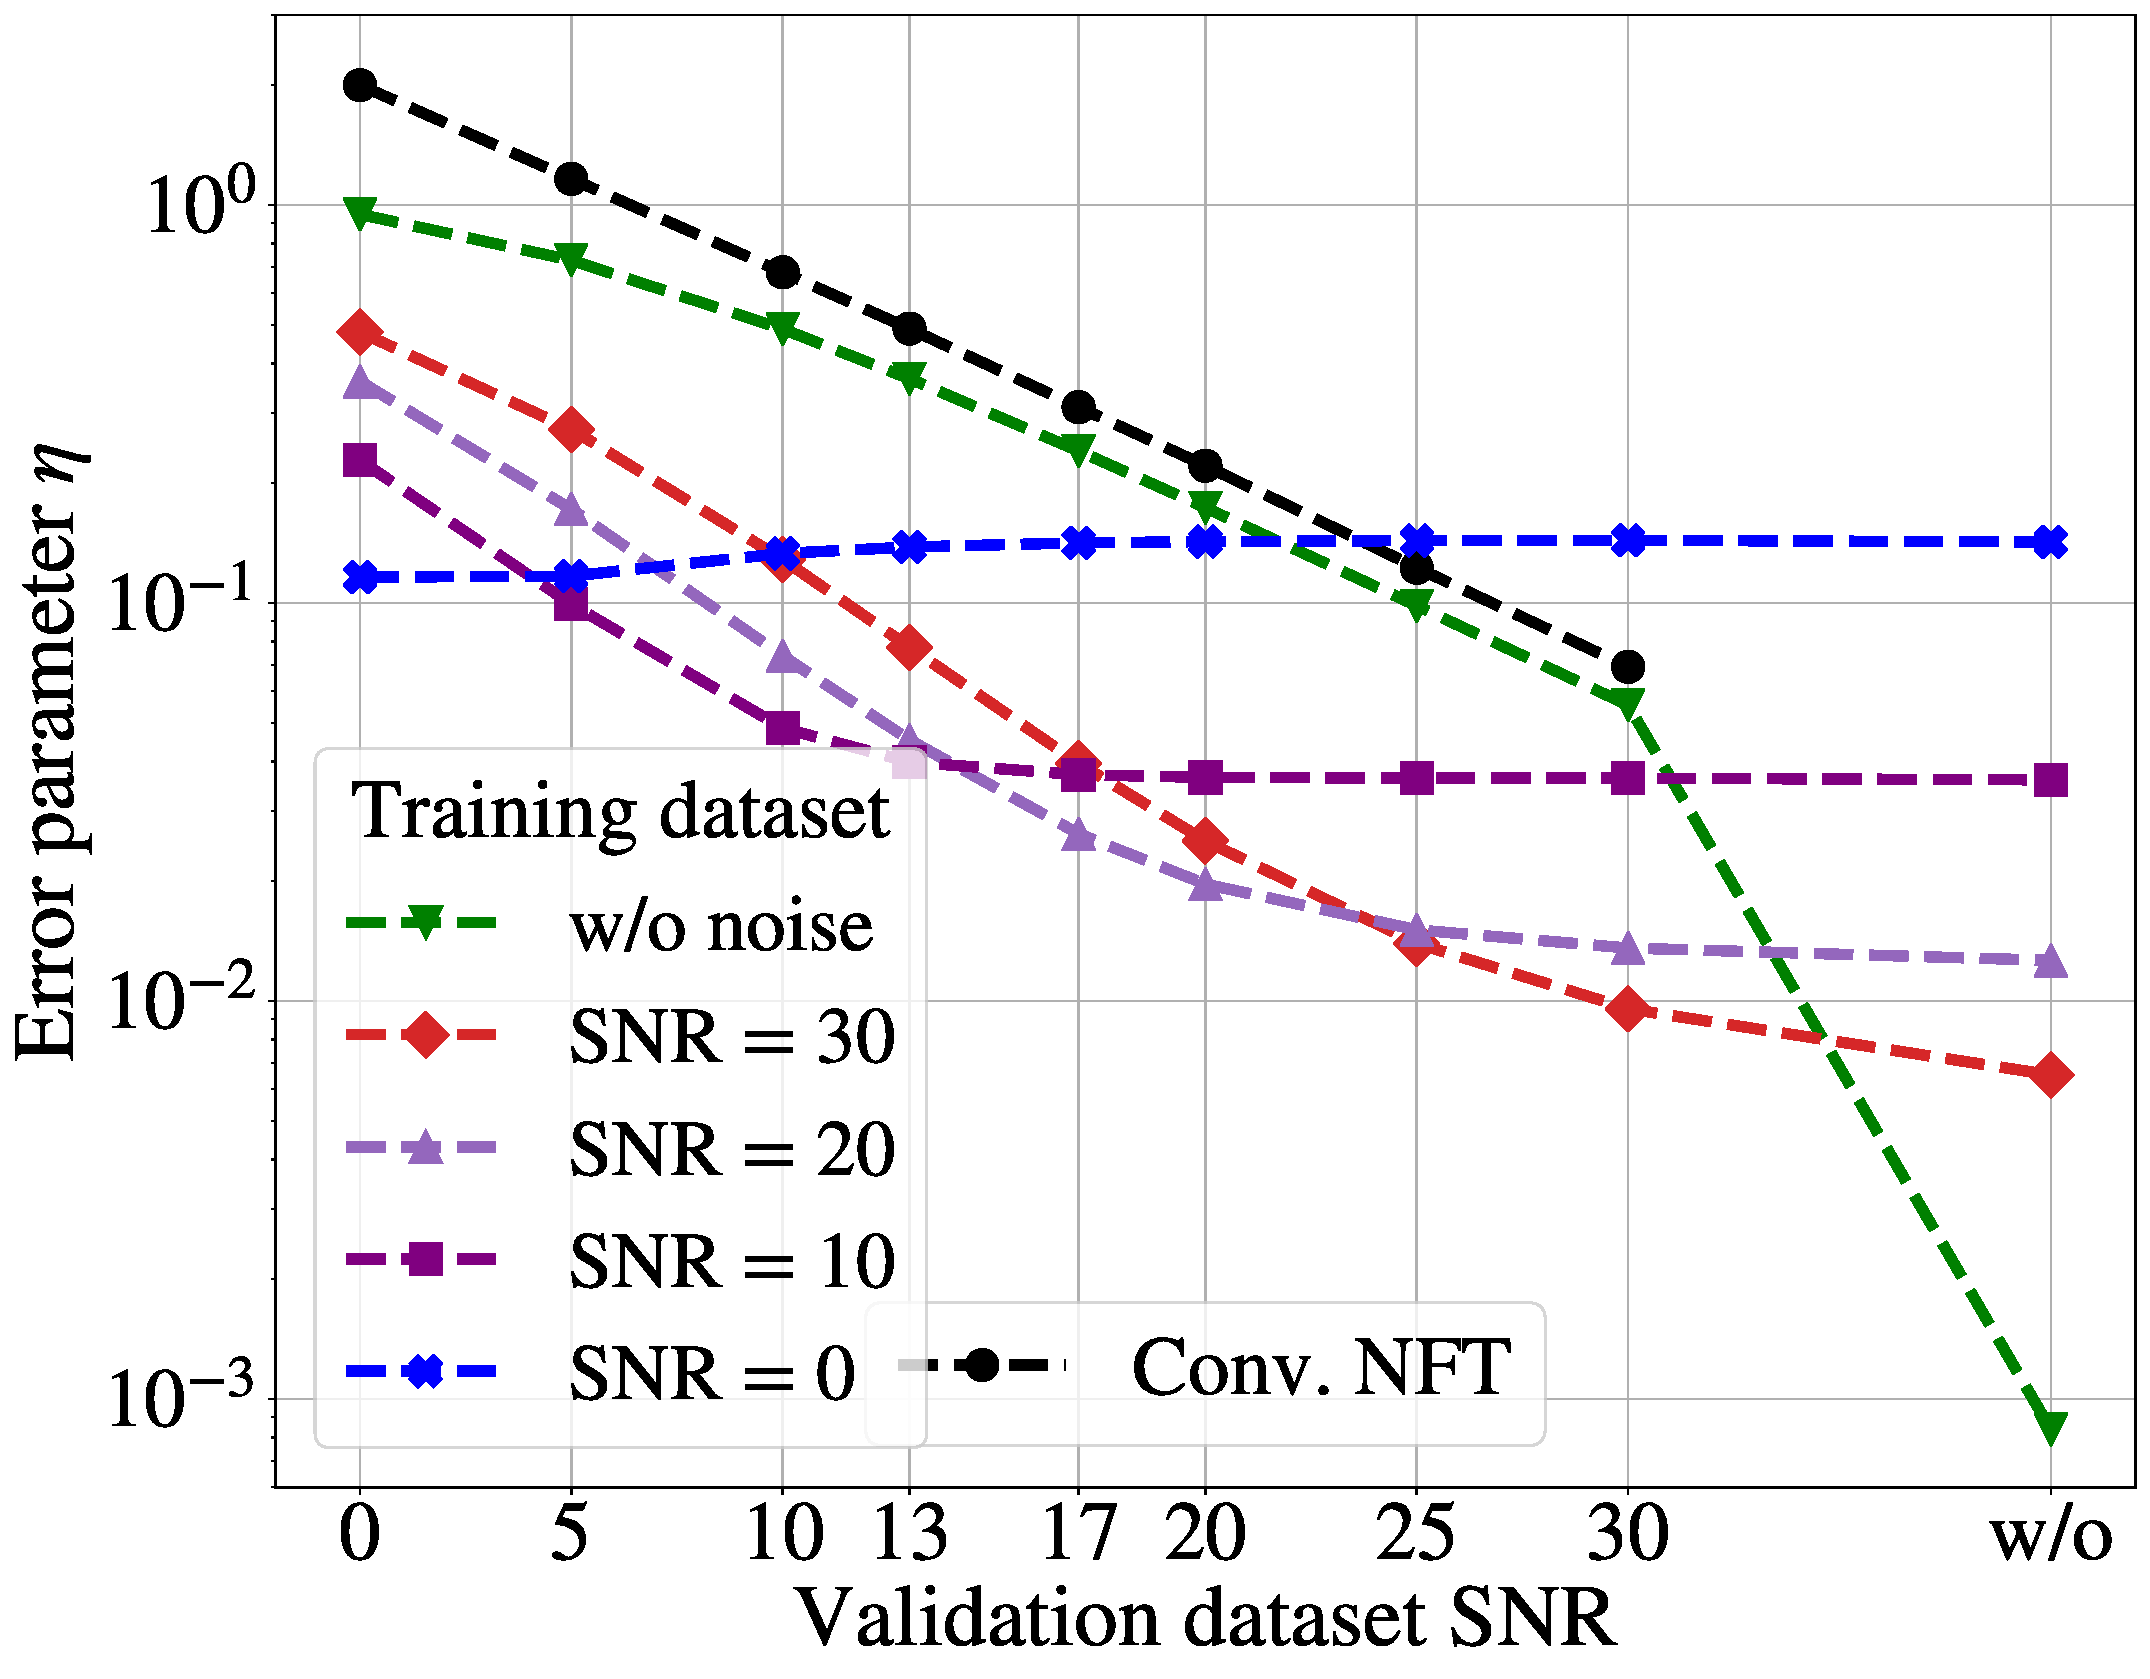
\includegraphics[width=1.\linewidth]{images/nn_nft/scirep_nft_r_metric.pdf}
  \caption{}
  \label{fig:quality_r}
\end{minipage}%
\begin{minipage}{.49\textwidth}
  \centering
  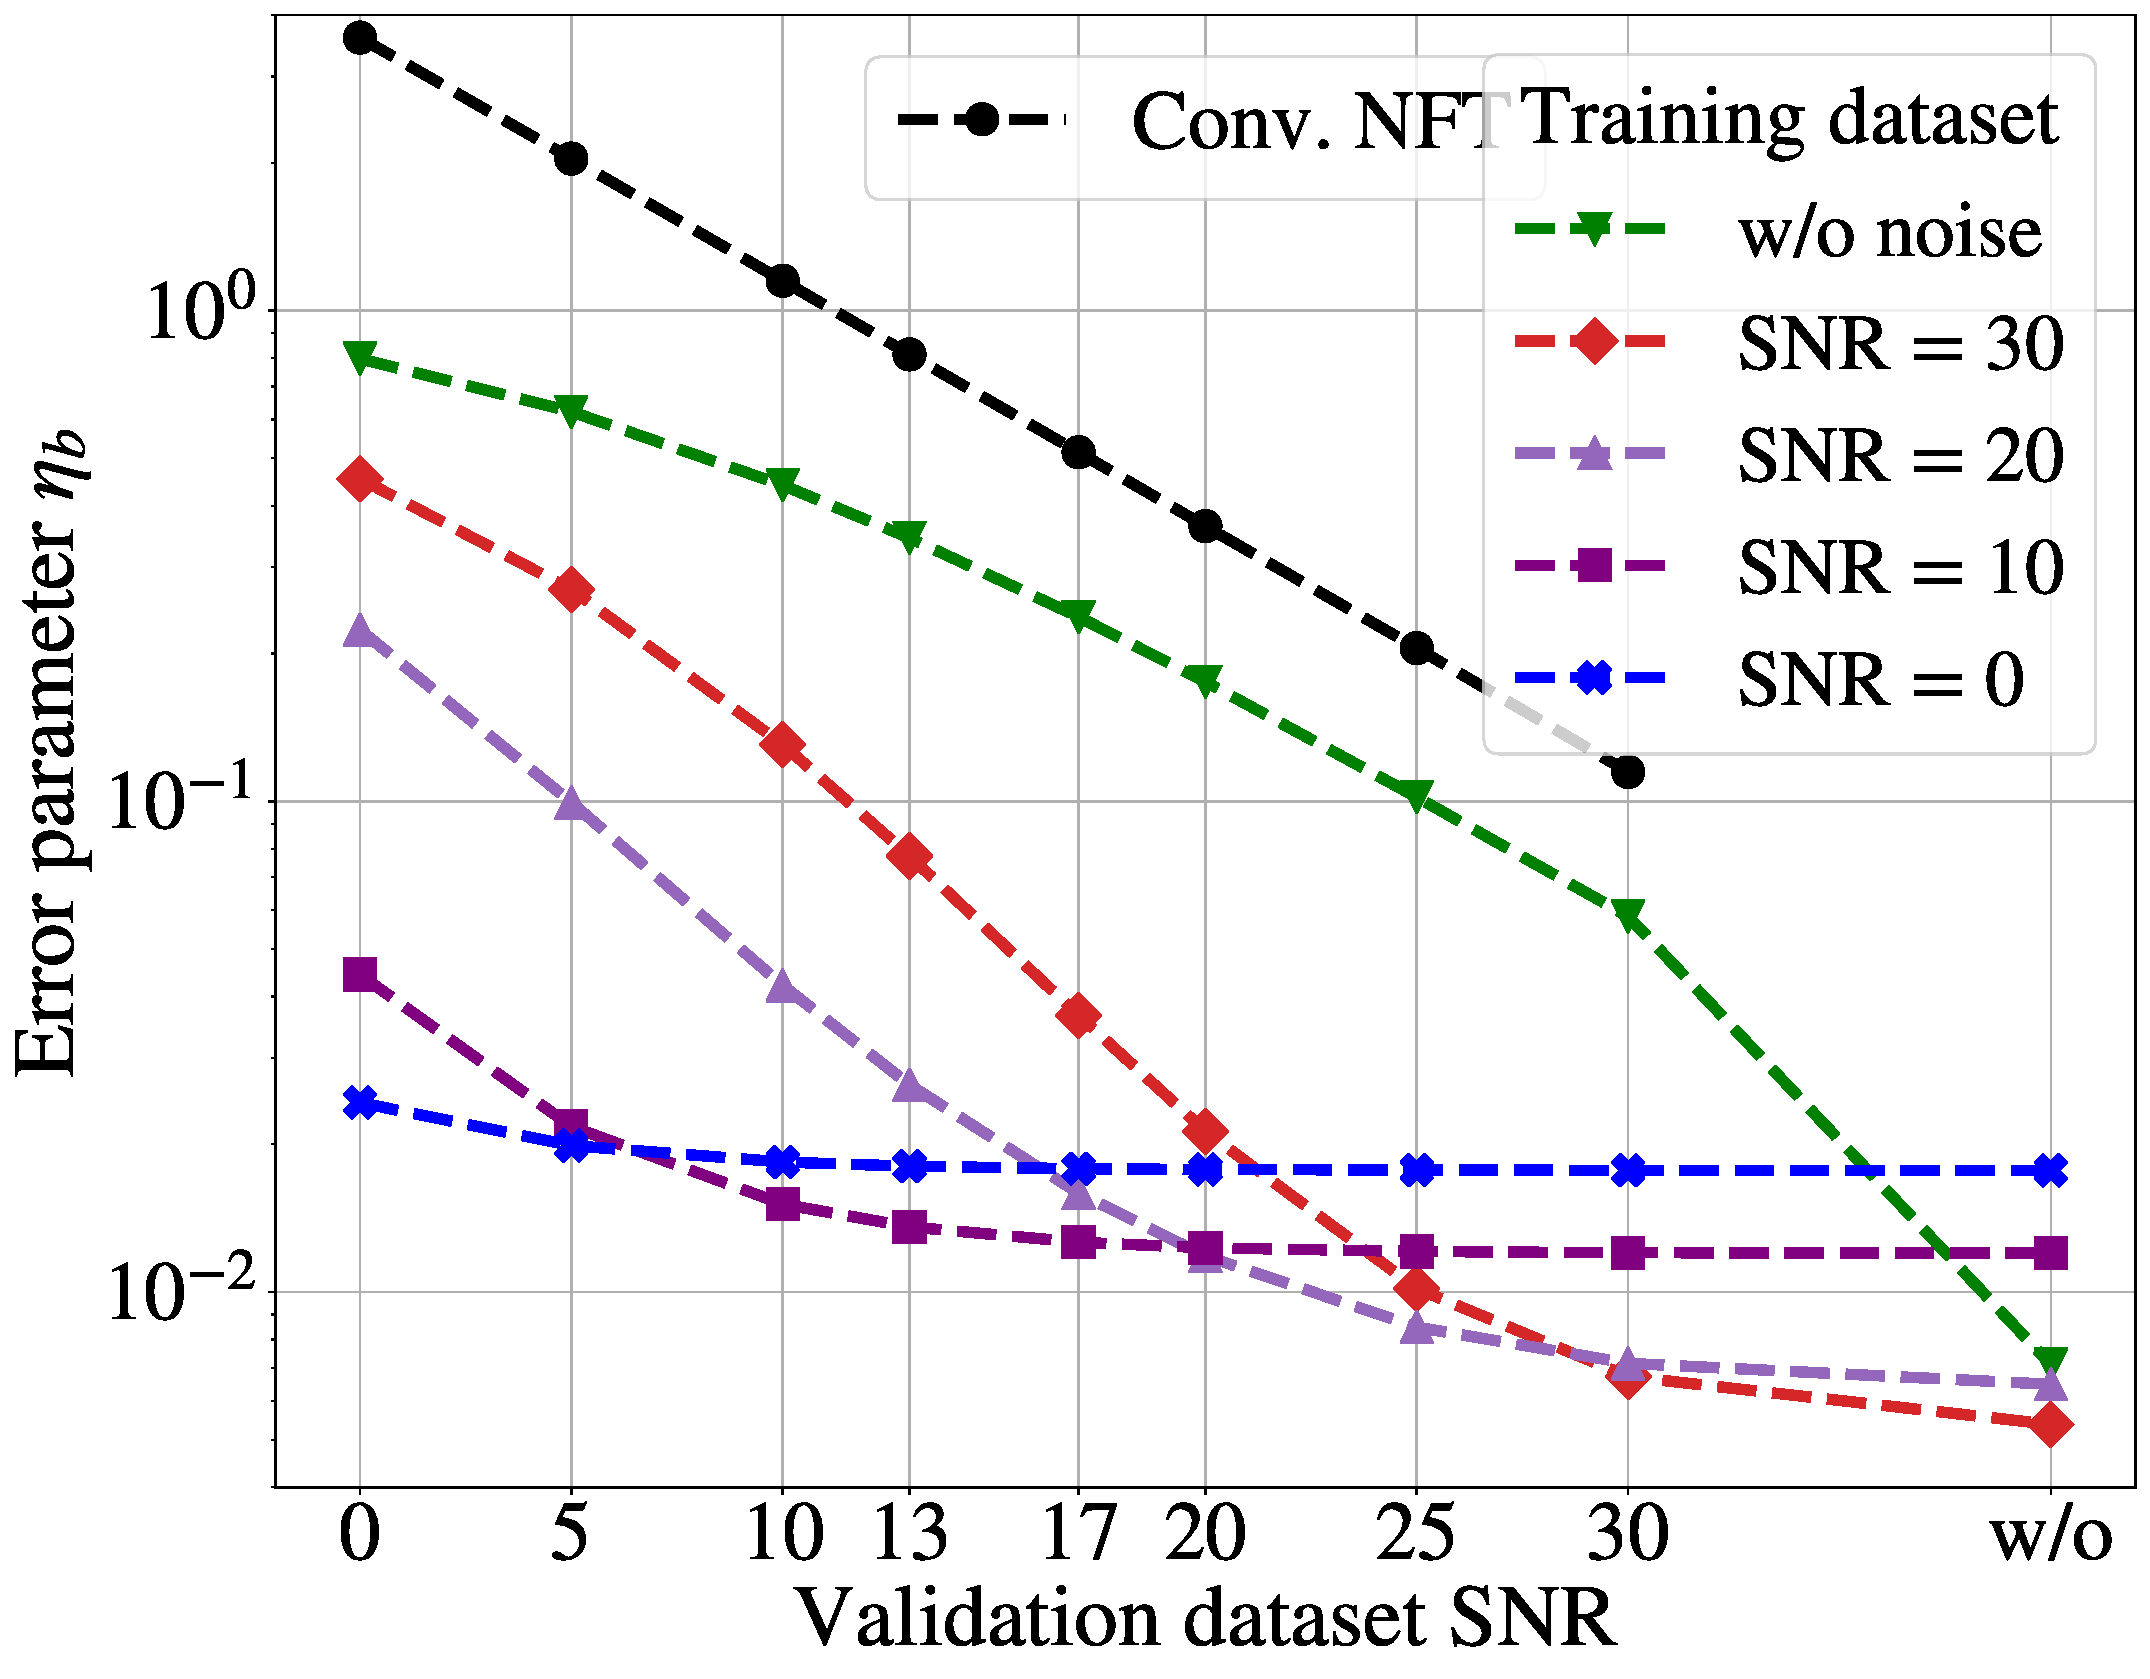
\includegraphics[width=1.\linewidth]{images/nn_nft/scirep_nft_b_metric.pdf}
  \caption{}
  \label{fig:quality_b}
\end{minipage}
\caption{\textbf{(a)} The dependence of the error parameter $\eta$~(\ref{eq:metric}) for coefficient $r(\xi)$ on the SNR value of the validation dataset for fast conventional NFT and NFT-Net trained at different noise levels. \textbf{(b)} The same for the error parameter $\eta_b$~(\ref{eq:b_metric}) for coefficient $b(\xi)$. The black line represents the error value for fast NFT applied to noisy signals, and the points below this line refer to the cases when the NFT-Net outperforms conventional computations. Other lines show  the value of the error in calculating the continuous spectrum using NFT-Net, trained with different noise levels: green -- without additional noise, red -- with additional noise with SNR = 30 dB, violet -- at SNR = 20 dB purple -- at SNR = 10 dB, blue -- at SNR = 0 dB.}
\label{fig:quality_r_b}
\end{figure}